\chapter{On Anomaly Ranking and Excess-Mass Curves}
\label{aistat:chap}
\begin{chapabstract}
This chapter presents the details relative to the introducing section~\ref{resume:scoring}.

Learning how to rank multivariate unlabeled observations depending on their degree of abnormality/novelty is a crucial problem in a wide range of applications. In practice, it generally consists in building a real valued `scoring' function on the feature space
so as to quantify to which extent observations should be considered as abnormal.
 In the 1-d situation, measurements are generally considered as `abnormal' when they are remote from central measures such as the mean or the median. Anomaly detection then relies on tail
analysis of the variable of interest. Extensions to the multivariate setting are far from straightforward and it is precisely the main purpose of this chapter to introduce a novel and convenient (functional) criterion for measuring the performance of a scoring function regarding the anomaly ranking task, referred to as the \textit{Excess-Mass} curve ($EM$
curve). In addition, an adaptive algorithm for building a scoring function based on unlabeled data $X_1,\; \ldots,\; X_n$ with a nearly optimal $EM$-curve is proposed and is analyzed from a statistical perspective.
\end{chapabstract}
Note: The material of this chapter is based on previous work published in \cite{AISTAT15}.



\section{Introduction}

In a great variety of applications  (\textit{e.g.} fraud detection, distributed fleet monitoring, system management in data centers), it is of crucial importance to address anomaly/novelty issues from a ranking point of view. In contrast to novelty/anomaly detection (\textit{e.g.} \cite{Kolt97, VertVert, Scholkopf2001, SHS05}), novelty/anomaly ranking is very poorly documented in the statistical learning literature (see \cite{VCTWMS} for instance). However, when confronted with
massive data, being enable to rank observations according to their supposed
degree of abnormality may significantly improve operational processes and allow for a prioritization of actions to be taken, especially in situations where human expertise required to check each observation is time-consuming.
% \par
When univariate, observations are usually considered as `abnormal'
when they are either too high or else too small compared to central
measures such as the mean or the median. In this context, anomaly/novelty analysis generally relies
on the analysis of the tail distribution of the variable of interest.  No natural (pre)~order exists on a $d$-dimensional feature space,  $\mathcal{X} \subset\mathbb{R}^d$ say, as soon as $d>1$. Extension to the multivariate setup is thus far from obvious and, in practice, the optimal ordering/ranking must be \textit{learned} from training data $X_1,\; \ldots,\; X_n$, in absence of any parametric assumptions on the underlying probability distribution describing the `normal' regime. The most straightforward manner to define a preorder on the feature space $\mathcal{X}$ is to transport the natural
order on the real half-line through a measurable \textit{scoring
  function} $s:\mathcal{X} \rightarrow \mathbb{R}_+$: the
`smaller' the score $s(X)$, the more `abnormal' the observation $X$ is
viewed. In the following, to simplify notation we assume that $\mathcal{X} = \rset^d$.
%
The whys and wherefores of scoring functions have been explained in the introduction chapter, Section~\ref{resume:scoring_function}. Estimating good scoring functions is a way to estimate level sets of the underlying density, as optimal scoring function are those whose induced level sets are exactly the ones of the density. The basic idea is that we don't need to estimate the density to obtain such level sets, but only any increasing transform of the density.
%
Any scoring function defines a preorder on $\rset^d$ and thus a ranking on a set of new observations. An important issue stated in Section~\ref{resume:scoring_function} concerns the definition of an adequate performance criterion, $\crit(s)$ say, in order to compare possible candidate scoring function and to pick one eventually: optimal scoring functions $s^*$ being then defined as those optimizing $\crit$. 
Estimating scoring function instead of the density itself precisely allows to use an other criterion than the distance to the density, which is too stringent for a level sets estimation purpose: a function having exactly the same level sets as the density can be very far from the latter using such distance.

Throughout the present article, it is assumed that the distribution $F$ of the observable \rv~$X$ is absolutely continuous \wrt~Lebesgue measure $\leb$ on
$\rset^d$, with density $f(x)$.  The criterion should be thus defined in a way that the collection of level sets of an optimal scoring function $s^*(x)$ coincides with that related to $f$.  In other words, any nondecreasing transform of the density should be optimal regarding the ranking performance criterion $\crit$. According to the Empirical Risk Minimization (ERM) paradigm, a scoring function will be built in practice by optimizing an empirical version $\crit_n(s)$ of the
criterion over an adequate set of scoring functions $\S_0$ of controlled complexity (\textit{e.g.} a major class of finite {\sc VC} dimension). Hence, another desirable property to guarantee the universal consistency of ERM learning strategies is the uniform convergence of
$\crit_n(s)$ to $\crit(s)$  over such collections $\S_0$ under minimal assumptions on the distribution $F(dx)$.

As described in Section~\ref{resume:mv-curve}, a functional criterion referred to as the mass-volume curve ($MV$-curve), admissible with respect to the requirements listed above has been introduced in \cite{CLEM13}, extending somehow the concept of $\roc$ curve in the unsupervised setup. Relying on the theory of \textit{minimum volume} sets (see Section~\ref{resume:mv-set}), it has been proved that the scoring functions minimizing empirical and discretized versions of the $MV$-curve criterion are accurate when the underlying distribution has compact support and a first algorithm for building nearly optimal scoring functions, based on the estimate of a finite collection of properly chosen minimum volume sets, has been introduced and analyzed. 
However, as explained in Section~\ref{resume:mv-curve}, some important drawbacks are inherent to this mass-volume curve criterion:
\begin{itemize}
\item[\textbf{1)}] When used as an performance criterion, the lebesgue measure of possibly very complex sets has to be computed.
\item[\textbf{2)}] When used as an performance criterion, the pseudo-inverse $\alpha_s^{-1}(\alpha)$ may be hard to compute.
\item[\textbf{3)}] When used as a learning criterion (in the ERM paradigm), it produces level sets which are not necessarly nested, on which may be built inaccurate scoring function. 
\item[\textbf{4)}] When used as a learning criterion, the learning rates are rather slow (of the order $n^{-1/4}$ namely), and cannot be established in the unbounded support situation.
\end{itemize}
 % See Figure~\ref{aistat:algo-problem} and related comments for an insight into the gain resulting from the concept introduced in the present paper in contrast to the $MV$ curve minimization approach relatively to the . 
 Given these limitations, it is the major goal of this chapter to propose an alternative criterion for anomaly ranking/scoring, called the \textit{Excess-Mass} curve ($EM$ curve in short) here, based on the notion of {\it density contour clusters}  \cite{Polonik95,Hartigan1987,Muller1991}. Whereas minimum volume sets are solutions of volume minimization problems under mass constraints, the latter are solutions of mass maximization under volume constraints. Exchanging this way objective and constraint, the relevance of this performance measure is thoroughly discussed and accuracy of solutions which optimize statistical counterparts of this criterion is
investigated. More specifically, rate bounds of the order $n^{-1/2}$ are proved, even in the case of unbounded support. Additionally, in contrast to the analysis carried out in \cite{CLEM13}, the model bias issue is tackled,
insofar as the assumption that the level sets of the underlying
density $f(x)$ belongs to the class of sets used to build the scoring
function is relaxed here. 

 The rest of this chapter is organized as follows. Section~\ref{aistat:sec:notations} introduces the notion of $EM$ curve and that of optimal $EM$
curve. Estimation in the compact support case is covered by Section~\ref{aistat:sec:estim}, extension to distributions with non compact support and
control of the model bias are tackled in Section~\ref{aistat:sec:ext}. A simulation study is
performed in Section~\ref{aistat:sec:simul}. All proofs are deferred to the
last section~\ref{aistat:sec:detailed_proofs}.   


% The convergence rates obtained with the EM
% criterion are faster than the one concerning here 

%  The
% criterion we promote here is referred to as the \emph{Excess-Mass
%   Curve} (\emph{EM curve} in short),  with
% the Mass-Volume Curve introduced in \cite{CLEM13}. We will see that it
% leads to scoring functions with stronger convergence rates while
% weakening assumptions.

% Given a class $\mathcal{G}$ of borelian subsets of $X$,  a minimum
% volume set $\Omega^*_{\alpha}$ over $\mathcal{G}$, of mass at least $\alpha\in(0,1)$, is any solution of the constrained minimization problem
% \begin{align}
% \label{aistat:MV}
%  \min_{\Omega\in\mathcal{G}}\leb(\Omega) \mbox{~~subject to~~}
%  F(\Omega)\geq \alpha\,.
% \end{align}
% The value of minimum is denoted $MV_{\mathcal{G}}(\alpha)$. Abnormal observations are those which belong to %the complementary set
% $\rset^d\setminus\Omega^*_{\alpha}$, for some large value  of
% $\alpha$. 

\section{Background and related work} \label{aistat:sec:background}
As a first go, we first recall the $MV$ curve criterion approach as introduced in Section~\ref{resume:mv-curve},
% provide a brief overview
% of the scoring approach based on  the $MV$ curve criterion,
as a basis
for comparison with that promoted in the present contribution.

% Here and throughout, the indicator function of any event $\mathcal{E}$ is denoted by $\mathds{1}_{\mathcal{E}}$, the Dirac mass at any point $x$ by $\delta_x$, $A\Delta B$ the symmetric difference between two sets $A$ and $B$ and by 

Recall that $\mathcal{S}$ is the set of all scoring functions
$s: \rset^d \rightarrow \mathbb{R}_+ $ integrable \wrt~Lebesgue
measure.
Let $s\in \mathcal{S}$. As defined in \cite{CLEM13,CLEM14}, the
$MV$-curve of $s$ is the plot of the mapping $$\alpha\in (0,1)\mapsto MV_s(\alpha) = \lambda_s \circ \alpha_s^{-1}(\alpha),$$
where 
\begin{equation}
\begin{aligned}
\label{aistat:eq:alpha}
\alpha_s(t) &= \mathbb{P}(s(X) \ge t),\\ 
\lambda_s(t) &=\leb(\{x \in \rset^d, s(x) \ge t\})
  \end{aligned}
\end{equation}

 and $H^{-1}$ denotes the pseudo-inverse of any cdf $H:\mathbb{R}\rightarrow (0,1)$.
%
This induces a partial ordering on the set of all scoring functions: $s$ is
preferred to $s'$ if $MV_{s}(\alpha) \le MV_{s'}(\alpha)$ for all
$\alpha\in(0,1)$.
One may show that $MV^*(\alpha)\leq MV_s(\alpha)$ for all $\alpha\in (0,1)$ and any scoring function $s$, where $MV^*(\alpha)$ is the optimal value of the constrained minimization problem
\begin{equation}\label{aistat:eq:MV}\min_{\Gamma~ borelian} ~\leb(\Gamma) \mbox{~subject to~} \mathbb{P}(X \in \Gamma) \ge \alpha.
\end{equation}
Suppose now that $F(dx)$ has a density $f(x)$ satisfying the following assumptions:

\noindent $\mathbf{A_1}$ {\it The density $f$ is bounded, \textit{i.e.} $\vert \vert f(X)\vert\vert_{\infty}<+\infty~.$} \\
\noindent $\mathbf{A_2}$ {\it The density $f$ has no flat parts: $\forall c\geq 0$, $\mathbb{P}\{f(X)=c\}=0~.$}\\~\\
 One may then show that the curve $MV^*$ is actually a $MV$ curve, that is related to (any increasing transform of) the density $f$ namely: $MV^*=MV_f$. In addition, the  minimization problem \eqref{aistat:eq:MV} has a unique solution
$\Gamma_\alpha^*$ of mass $\alpha$ exactly, referred to as \textit{minimum volume set} (see Section~\ref{resume:mv-set}): $$MV^*(\alpha)=\leb(\Gamma^*_\alpha) ~~~\text{and}~~~ F(\Gamma_\alpha^*)=\alpha .$$ Anomaly scoring can be then viewed as the problem of building a scoring function $s(x)$ based on training data such that $MV_s$ is (nearly) minimum everywhere, \textit{i.e.} minimizing $$\|MV_{s}-MV^*\|_{\infty}:=\sup_{\alpha\in[0,1]}\vert MV_s(\alpha)-MV^*(\alpha)\vert.$$
% The minimizer $\Omega_\alpha^*$ is a \emph{minimum volume set}.%, where $\Omega_\alpha^*$.%  is
% any solution of the above minimization problem.
% and that in the case where $g$ is a nondecreasing transform of $f$, $MV_g=MV^*$.\\
% Under assumptions $\mathbf{A}_1$-$\mathbf{A}_2$, $MV^*$ is continuous on $(0,1)$ and uniformly continuous on $[0,1-\epsilon]$ for all $\epsilon \in (0,1)$ (when the support of $F(dx)$ is compact, uniform continuity holds on the whole interval $[0,1]$).
Since $F$ is unknown, a minimum volume set estimate $\widehat{\Gamma}^*_{\alpha}$ can be defined as the solution of \eqref{aistat:eq:MV} when $F$ is replaced by its empirical version
$F_n=(1/n)\sum_{i=1}^n\delta_{X_i}$, minimization is restricted to a collection $\mathcal{G}$ of borelian subsets of $\rset^d$ supposed not too complex but rich enough to include all density level sets (or reasonable approximants of the latter) and $\alpha$ is replaced by $\alpha-\phi_n$, where the {\it tolerance parameter} $\phi_n$ is a probabilistic upper bound for the supremum $\sup_{\Gamma\in \mathcal{G}}\vert F_n(\Gamma)-F(\Gamma) \vert$. Refer to \cite{Scott2006} for further details. The set $\mathcal{G}$ should ideally offer statistical and computational advantages both at the same time. Allowing for fast search on the one hand and being sufficiently complex to capture the geometry of target density level sets on the other.
%: $\inf_{\Omega \in \mathcal{G}} \leb(\Omega \Delta \Omega^*_\alpha )$ should be small for any $\alpha$, $\Delta$ denoting the symmetric difference.
In \cite{CLEM13}, a method consisting in preliminarily estimating a collection of minimum volume sets related to target masses $0<\alpha_1<\ldots<\alpha_K<1$ forming a subdivision of $(0,1)$ based on training data so as to build a scoring function $$s=\sum_k \mathds{1}_{x\in \hat \Gamma_{\alpha_k}^*}$$ has been proposed and analyzed. Under adequate assumptions (related to $\mathcal{G}$, the perimeter of the $\Gamma^*_{\alpha_k}$'s and the subdivision step in particular) and for an appropriate choice of $K=K_n$ either under the very restrictive assumption that $F(dx)$ is compactly supported or else by restricting the convergence analysis to $[0,1-\epsilon]$ for $\epsilon>0$, excluding thus the tail behavior of the distribution $F$ from the scope of the analysis, rate bounds of the order $\mathcal{O}_{\mathbb{P}}(n^{-1/4})$ have been established to guarantee the generalization ability of the method.

Figure~\ref{aistat:algo-problem} illustrates one problem inherent to the use of the $MV$ curve as a performance criterion for anomaly scoring in a `non asymptotic' context, due to the prior discretization along the mass-axis. In the $2$-d situation described by Figure~\ref{aistat:algo-problem} for instance, given the training sample and the partition of the feature space depicted, 
%choosing the subdivision $0,\; 1/2,\; 11/20,\; 1$
the $MV$ criterion leads to consider the sequence of empirical minimum volume sets $A_1,\; A_1\cup A_2,\; A_1\cup A_3,\; A_1\cup A_2\cup A_3$ and thus the scoring function $s_1(x)=\mathbb{I}\{x\in A_1  \}+ \mathbb{I}\{x\in A_1\cup A_2  \} + \mathbb{I}\{x\in A_1\cup A_3  \}$, whereas the scoring function $s_2(x)=\mathbb{I}\{x\in A_1  \}+ \mathbb{I}\{x\in A_1\cup A_3  \}$ is clearly more accurate.
%The objective is then to  depending on the data $X_1,...X_n$ such that $\|MV_{s}-MV^*\|_{\infty}$ is minimal. Practically, $ s$ will be %of type $\sum_k \mathds{1}_{x\in \hat \Omega_{\alpha_k}^*}  $ where $(\alpha_k)$ is a subdivision of $[0,1[$.\\
%The MV-curve criterion leads to two main results, depending on the finite or infinite size of $supp f$ :\\\\
%In the finite case and under assumptions $\mathbf{A_1}$ -
%$\mathbf{A_2}$ , and other assumptions on the perimeter of $\partial
%\Omega^*_\alpha$, on the class of $MV^*$ and on the boundedness of
%$MV^{*'}$, one may construct $ s$  such that with probability at least $1-\delta$ :
%\begin{align} 
%\|MV_{ s}-MV^*\|_{\infty, \alpha \in [0,1]} \le A~ \log(1/\delta) \left(\frac{1}{K^2} + \sqrt{\frac{B+log K}{n}}\right)\,,
%\end{align}
%where $K$ is the step of the subdivision $\alpha_k$ on which $s$ is built.\\
%In the infinite case, under additional assumptions  $\mathbf{A_3}$ - $\mathbf{A_4}$ (specified later in this paper)
%it is possible to construct $ s$ such that with probability at least
%$1-\delta$,  
%\begin{align}
%\|MV_{ s}-MV^*\|_{\infty, \alpha \in [0,1-\epsilon]} \le \frac{c(\epsilon,\delta)}{n^{1/4}}\,.
%\end{align}
%Unfortunately, the constant $c(\epsilon,\delta)$ tends to infinity as
%$\epsilon \rightarrow 0$ which forbids the  use of  this bound  for evaluating the quality of $s$ in the tail of the distribution.
\par In this work, a different functional criterion is proposed, obtained by exchanging objective and constraint functions in \eqref{aistat:eq:MV}, and it is shown that optimization of an empirical discretized version of this performance measure yields scoring rules with convergence rates of the order $\mathcal{O}_{\mathbb{P}}(1/\sqrt{n})$. In addition, the results can be extended to the situation where the support of the distribution $F$ is not compact.
%The subsequent optimal scoring function
%enjoys stronger convergence properties and a speed of convergence in
%$\frac{1}{\sqrt n}$. The   upper bound's dependance on $\epsilon$  is
%removed, which enables an extension to  the entire (infinite) support
%of $f$, namely on a set of possible mass $1$ instead of
%$1-\epsilon$. Finally, the bias of the new  model is controlled  by a
%simple bound, which can be made as small as desired by refining the discretization.


\section{The Excess-Mass curve}\label{aistat:sec:notations}
As introduced in Section~\ref{resume:em-curve}, the performance criterion we propose in order to evaluate anomaly scoring accuracy relies on 
the notion of \textit{excess mass} and \textit{density contour
clusters}, as introduced in the seminal contribution \cite{Polonik95}. The main idea is to consider a Lagrangian formulation of a constrained minimization problem, obtained by exchanging constraint and objective in \eqref{aistat:eq:MV}: for $t>0$,
\begin{equation}
\label{aistat:solomeg}
\max_{\Omega~ borelian}  \left\{ \mathbb{P}(X \in \Omega) - t \leb(\Omega) \right\}.
\end{equation}
We denote by $\Omega^*_t$ any solution of this problem. As shall be seen in the subsequent analysis  (see Proposition~\ref{aistat:propmono}
 below), compared to the $MV$ curve approach, this formulation offers certain computational and theoretical advantages both at the same time: when letting (a discretized version of) the Lagrangian multiplier $t$ increase from $0$ to infinity, one may easily obtain solutions of empirical counterparts of \eqref{aistat:solomeg} forming a \textit{nested} sequence of subsets of the feature space, avoiding thus deteriorating rate bounds by transforming the empirical solutions so as to force monotonicity.
 %This can be explained by the fact that a mass constraint introduces an additional discretization dimension (along the distributional mass) which is a priori independent of the volume discretization resulting from the (countable number of) empirical clusters. 
% is to solve a volume
%penalization problem instead of one constrained by the mass $\alpha$.
%Indeed, a mass constraint introduces an additional
%discretization dimension (along the distributional mass) % an other
% `discretization's dimension' along $\alpha$,
% which is a priori independent of the volume discretization  \emph{a priori} 
% resulting from the choice of a class $\mathcal{G}$. {\blue je voulais plutot dire que la discretisation en volume était nécessaire car on ne peut résoudre qu'un nombre dénombrable de problèmes d'optimisation (on est obligé d'avoir un nombre dénombrable de solutions empirique $\hat \Omega_i,i \in \mathbb{N}$)} % of  the
%  (empirical) level sets 
% for the optimization problem - which leads to a discretization in the volume of such sets, not in their mass. 
% Instead, penalizing the  volume of such sets % - namely the more one penalizes the volume, the more concentrated will be the level set -
%is deeply related  with the volume discretization and enables  better
% control of the empirical level sets (see proposition~\ref{aistat:propmono}
 %later), \emph{via} an adaptive penalization (see Section
 %\ref{aistat:sec:infiniteSupport})
%\noindent
% Analogously to the previous subsection, $X$ being a random variable on
% $\mathcal{X} \subset \mathcal{R}^d$ and $\leb$ denoting the \lebesgue
% measure on $\mathbb{R}^d$, c
%\par Consider, for any $t>0$, the  optimization problem
%
%\noindent
 %nd denote by $\Omega_t^*$ any solution. Equation~\ref{aistat:solomeg} can
%be interpreted as a  Lagrangian formulation  of \eqref{aistat:MV}, with a linear
%penality $t$ on the volume instead of the mass. 
%Define subsequently the optimal Excess
%Mass curve as :
\begin{definition}\label{aistat:def:opt}{\sc (Optimal $EM$ curve)} The optimal Excess-Mass curve related to a given probability distribution $F(dx)$ is defined as the plot of the mapping $$t>0\mapsto EM^*(t):=\max_{\Omega\text{ borelian} } \{ {\mathbb{P}} (X\in \Omega)-t\leb(\Omega) \}.$$ 
%\begin{equation*}
%EM^*(t):=  \mathbb{P}(X \in \Omega_t^*)-t.\leb(\Omega_t^*)  = \max_{\Omega~ mes.} \mathbb{P}(X \in \Omega)-t.\leb(\Omega) 
%\end{equation*}
\end{definition}
Equipped with the notation above, we have: $EM^*(t)=\mathbb{P}(X \in \Omega_t^*)-t \leb(\Omega_t^*)$ for all $t>0$.
Notice also that $EM^*(t) = 0$ for any $t>\|f\|_\infty:=\sup_{x\in \rset^d}\vert f(x)\vert$. 
% &\mbox{i.e.~~} &&\forall~ t \in [0,\|f\|_\infty],~ EM^*(t)=\max_{\Omega mes.} \mathbb{P}(X \in \Omega)-t.\leb(\Omega) \\
% &\mbox{~~and~~} &&\forall~ t ~>~ \|f\|_\infty,~ EM^*(t)=0
% The following lemma characterizes $\Omega_t^*$. % when   assumption
 % $\mathbf{A_2}$ holds true.

\begin{figure}[!ht]
\centering
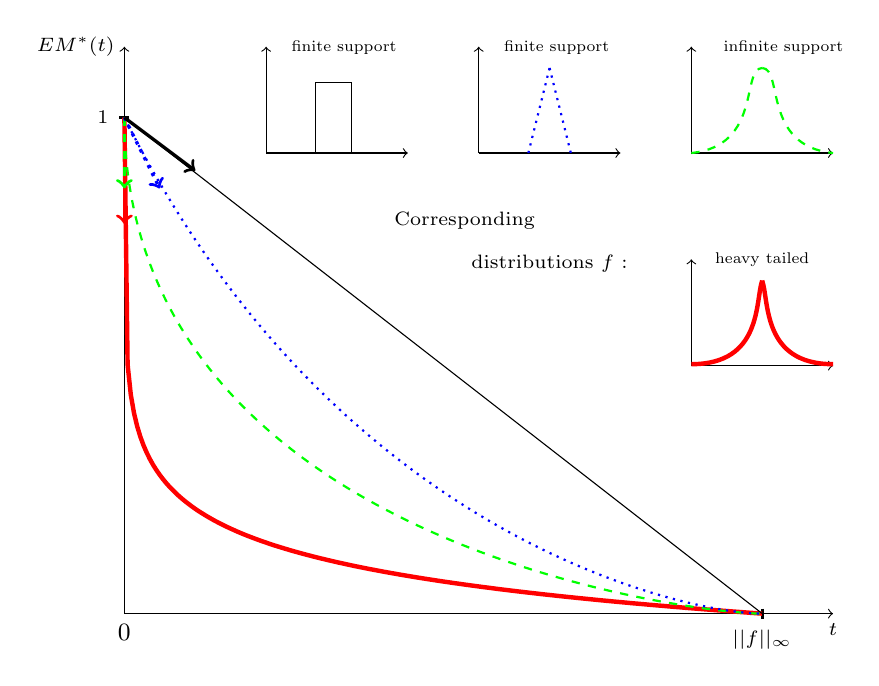
\begin{tikzpicture}[scale=0.9]


\newcommand*{\maxx}{10}
\newcommand*{\maxy}{7}
\newcommand*{\maxf}{9}

%axes:
\draw[->](0,0)--(\maxx,0) node[below]{\scriptsize $t$};
\draw[->](0,0)--(0,\maxy+1) node[left]{\scriptsize $EM^*(t)$}; 

\draw[very thick](\maxf,2pt)--(\maxf,-2pt) node[below]{\scriptsize  $||f||_\infty$} ;
\draw[very thick](2pt,\maxy)--(-2pt,\maxy) node[left]{\scriptsize  1} ;
\draw[very thick](0pt,0)--(0pt,0) node[below]{\small 0} ;

\draw (\maxx/2-0.2,\maxy/2+2.3) node[below]{\scriptsize  Corresponding} ;
\draw (\maxx/2+1,\maxy/2+1.7) node[below]{\scriptsize  distributions $f$ :} ;

%petits graphs
\draw[->](2,\maxy-0.5)--(4,\maxy-0.5) node[below]{};
\draw[->](2,\maxy-0.5)--(2,\maxy+1) node[left]{}; 
\draw (2.7,\maxy-0.5) ..controls +(0,1) and +(0,-1).. (2.7,\maxy +0.5);
\draw (2.7,\maxy+0.5) ..controls +(1,0) and +(-1,0).. (3.2,\maxy +0.5);
\draw (3.2,\maxy-0.5) ..controls +(0,1) and +(0,-1).. (3.2,\maxy +0.5);
\draw (3.1,\maxy+1.2) node[below][scale=0.8]{\scriptsize  finite support} ;
%\draw (2.4,\maxy) node[thick]{1} ;

\draw[->](5,\maxy-0.5)--(7,\maxy-0.5) node[below]{};
\draw[->](5,\maxy-0.5)--(5,\maxy+1) node[left]{}; 
\draw [blue, dotted, thick] (5.7,\maxy-0.5) ..controls +(0.3,1.2) and +(-0.3,-1.2).. (6,\maxy+0.7);
\draw [blue, dotted, thick] (6,\maxy+0.7) ..controls +(0.3,-1.2) and +(-0.3,1.2).. (6.3,\maxy-0.5);
\draw (6.1,\maxy+1.2) node[below][scale=0.8]{\scriptsize finite support} ;
%\draw (5.4,\maxy) node[thick]{2} ;

\draw[->](8,\maxy-0.5)--(10,\maxy-0.5) node[below]{};
\draw[->](8,\maxy-0.5)--(8,\maxy+1) node[left]{}; 
\draw [green, dashed, thick] (8,\maxy-0.5) ..controls +(1,0.1) and +(-0.3,-0.01).. (9,\maxy+0.7);
\draw [green, dashed, thick] (9,\maxy+0.7) ..controls +(0.3,-0.01) and +(-1,0.1).. (10,\maxy-0.5);
\draw (9.3,\maxy+1.2) node[below][scale=0.8]{\scriptsize  infinite support} ;
%\draw (8.4,\maxy) node[thick]{3} ;

\draw[->](8,\maxy-3.5)--(10,\maxy-3.5) node[below]{};
\draw[->](8,\maxy-3.5)--(8,\maxy-2) node[left]{}; 
\draw [red,ultra thick] (8,\maxy-3.48) ..controls +(1,0) and +(-0.1,-0.3).. (9,\maxy-2.3);
\draw [red,ultra thick] (9,\maxy-2.3) ..controls +(0.1,-0.3) and +(-1,0).. (10,\maxy-3.48);
\draw (9,\maxy-1.8) node[below][scale=0.8]{\scriptsize  heavy tailed} ;
%\draw (8.4,\maxy-3) node[thick]{4} ;

%EM curves:
\newcommand*{\aaa}{(1/sqrt(sqrt(\maxf))+1)}
\newcommand*{\bbb}{(-1/sqrt(sqrt(\maxf)))}

\draw [red,ultra thick,domain=0:\maxf, samples=200] plot (\x,{\maxy * (\aaa/(1+sqrt(sqrt(\x)))+\bbb)} ) ;
\draw [domain=0:\maxf, samples=200] plot (\x,{\maxy * (1- 1/\maxf * \x)} ) ;

\draw [green,dashed, thick] (0,\maxy) ..controls +(0,-6) and +(-1,0).. (\maxf,0); 
\draw [blue, dotted, thick] (0,\maxy) ..controls +(3,-6) and +(-1,0).. (\maxf,0); 

%tangentes:
\tikzstyle {tangente} = [very thick, ->];
\draw [tangente,red] (0,\maxy)--++( 0,-1.5);
\draw [tangente,green,dashed] (0,\maxy)--++( 0,-1);
\draw [tangente,blue,dotted] (0,\maxy)--++( 0.5,-1);
\draw [tangente] (0,\maxy)--++( 1,-0.75);

%legende figure
%\draw (\maxx/2,-1) node[thick]{Figure 3 : Excess Mass curves} ;

\end{tikzpicture}
\caption{EM curves depending on densities}
\label{aistat:EMcurves}
\end{figure}





\begin{center}
\begin{figure}
\centering
%\resizebox{8cm}{4cm}{
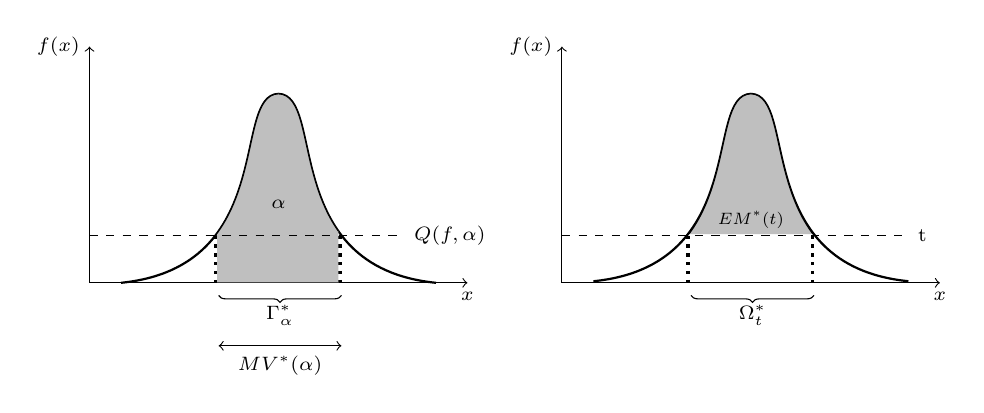
\begin{tikzpicture}[scale=2.]

\draw[->](7.8,0)--(10.2,0) node[below]{\scriptsize $x$};
\draw[->](7.8,0)--(7.8,1.5) node[left]{\scriptsize $f(x)$}; 
\draw [thick] (8,0) ..controls +(1,0.1) and +(-0.3,-0.01).. (9,1.2);
\draw [thick] (9,1.2) ..controls +(0.3,-0.01) and +(-1,0.1).. (10,0);

\draw[dotted,very thick](8.60,0.3)--(8.60,0) node[right]{};
\draw[dotted,very thick](9.39,0.3)--(9.39,0) node[right]{};

%\draw (8,0.3)--(10,0.3)--(10,1.5)--(8,1.5)--(8,0.3); dessine 4 segments correspondant au 4 points

%hachurage :
\begin{scope} 
\clip (8.61,0)--(9.38,0)--(9.38,1.5)--(8.61,1.5)--(8.61,0) ; %tout ce qui est dans begin{scope} se limitera au rectangle

\path[draw,fill=lightgray] (8,0) ..controls +(1,0.1) and +(-0.3,-0.01).. (9,1.2)--
(9,1.2) ..controls +(0.3,-0.01) and +(-1,0.1).. (10,0)--
(8,0)--(10,0) --cycle;
\end{scope}

\draw[dashed](7.8,0.3)--(9.8,0.3) node[right]{\scriptsize $Q(f,\alpha)$};

%accolade :
\draw[decorate,decoration={brace}]
(9.4,-0.08)--(8.62,-0.08) node[below,pos=0.5] {\scriptsize $\Gamma_\alpha^*$};

\draw[<->]
(9.4,-0.4)--(8.62,-0.4) node[below,pos=0.5] {\scriptsize $MV^*(\alpha)$};



\draw (9,0.5) node[thick]{\scriptsize $\alpha$} ;
%\draw (8.8,-0.8) node[thick]{Figure 1: MV curve} ;

\draw[->](10.8,0)--(13.2,0) node[below]{\scriptsize $x$};
\draw[->](10.8,0)--(10.8,1.5) node[left]{\scriptsize $f(x)$}; 
\draw [thick] (11,0.01) ..controls +(1,0.1) and +(-0.3,-0.01).. (12,1.2);
\draw [thick] (12,1.2) ..controls +(0.3,-0.01) and +(-1,0.1).. (13,0.01);
\draw[dashed](10.8,0.3)--(13,0.3) node[right]{\scriptsize t};
\draw[dotted,very thick](11.60,0.3)--(11.60,0) node[right]{};
\draw[dotted,very thick](12.39,0.3)--(12.39,0) node[right]{};

%\draw (8,0.3)--(10,0.3)--(10,1.5)--(8,1.5)--(8,0.3); dessine 4 segments correspondant au 4 points

%hachurage :
\begin{scope} 
\clip (11,0.31)--(13,0.308)--(13,1.5)--(11,1.5)--(11,0.308) ; %tout ce qui est dans begin{scope} se limitera au rectangle (8,0.3)--(10,0.3)--(10,1.5)--(8,1.5)--(8,0.3)
\path[draw,fill=lightgray] (11,0) ..controls +(1,0.1) and +(-0.3,-0.01).. (12,1.2)--
(12,1.2) ..controls +(0.3,-0.01) and +(-1,0.1).. (13,0)--
(11,0.3)--(13,0.3) --cycle;
\end{scope}

%accolade :
\draw[decorate,decoration={brace}]
(12.4,-0.08)--(11.62,-0.08) node[below,pos=0.5] {\scriptsize  $\Omega_t^*$};

\draw (12,0.4) node[scale=0.85]{\scriptsize $EM^*(t)$} ;
\draw (11.8,-0.5) node[thick]{ } ;
\end{tikzpicture}
%}
\caption{Comparison between $MV^*(\alpha)$ and $EM^*(t)$}
\label{aistat:MVcurve}
\end{figure}
\end{center}



\begin{lemma}{\sc (On existence and uniqueness)}
\label{aistat:evident}
For any subset $\Omega^*_t$ solution of \eqref{aistat:solomeg}, we have
$$\{x, f(x) > t\} ~\subset~ \Omega^*_t ~\subset~ \{x, f(x) \ge t\} \text{~~~~almost-everywhere},$$
 and the sets $\{x, f(x) > t\}$ and $\{x, f(x) \ge t\}$ are both solutions of \eqref{aistat:solomeg}.
In addition, under assumption $\mathbf{A_2}$, the solution is unique:% and we have 
$$\Omega_t^*~=~ \{x, f(x) > t\}~=~ \{x, f(x) \ge t\}.$$%% \quad \text{ is unique }$$
\end{lemma}
 Observe that the curve $EM^*$ is always well-defined,
since  $ \int_{f \ge t}(f(x)-t)dx = \int_{f > t}(f(x)-t)dx$. We also point out that $EM^*(t)=\alpha(t)-t\lambda(t)$ for all $t>0$, where we set $\alpha = \alpha_f$ and
$\lambda = \lambda_f$ where $\alpha_f$ and $\lambda_f$ are defined in \eqref{aistat:eq:alpha}. % where the mappings $\alph$ and
% $\lmabda$ are we recall the notation :
% \begin{align*}
% &\alpha_s (t):= \mathbb{P}(s(X)\geq t)~~~~~~~~~~~~~~~~~~~~~~~~~~~~~~~~ \\
% &\lambda_s(t):=\leb\{x \in \rset^d,s(x)\geq t\}\\
% \mbox{and}~~~~~~~~~~~~&\\
% &\alpha (t):= \alpha_f (t) \\
% &\lambda (t):=\lambda_f(t)
% \end{align*}
% \noindent
%As for the variational properties of the EM-curve, 
%The coarea formula for Lipschitz functions leads to the result stated below.
\begin{proposition}{\sc (Derivative and convexity of $EM^*$)}  Suppose that assumptions $\mathbf{A_1}$ and $\mathbf{A_2}$ are fullfilled. Then, the mapping $EM^*$ is differentiable and we have for all $t>0$:
\label{aistat:derive}
\begin{eqnarray*}
 EM^{*'}(t)=-\lambda(t). 
\end{eqnarray*}
In addition, the mapping $t>0 \mapsto \lambda(t)$ being decreasing, the curve $EM^*$ is convex.
\end{proposition}

We now introduce the concept of Excess-Mass curve of a scoring function $s\in \S$.
%The excess mass curve (EM curve) of  such scoring functions is a
%generalization of $EM^*$.
\begin{definition} {\sc ($EM$ curves)}
The  $EM$ curve of $s\in\mathcal{S}$  \wrt~the probability
distribution $F(dx)$ of a random variable $X$ is the plot of the mapping
\begin{equation}
\label{aistat:EM}
EM_s : t \in [0, \infty[ \mapsto \sup_{A \in \{(\Omega_{s,l})_{l>0}\}} {\mathbb{P}}(X \in A) - t \leb(A),
\end{equation}
where $\Omega_{s,t}=\{ x \in \rset^d, s(x) \ge t \}$ for all $t>0$.
One may also write: $\forall t>0$, $EM_s(t)= \sup_{u>0}~ \alpha_s(u) -
t \lambda_s(u) $. Finally, under assumption $\mathbf{A_1}$, we have $EM_s(t)=0$ for every $t> \|f\|_\infty$. 
\end{definition}


%\begin{figure}%{l}{65mm}
%\centering
%\begin{tikzpicture}[scale=1.5,width=4]
%
%\draw[->](7.8,0)--(10.2,0) node[below]{x};
%\draw[->](7.8,0)--(7.8,1.5) node[left]{f(x)}; 
%\draw [thick] (8,0.01) ..controls +(1,0.1) and +(-0.3,-0.01).. (9,1.2);
%\draw [thick] (9,1.2) ..controls +(0.3,-0.01) and +(-1,0.1).. (10,0.01);
%\draw[dashed](7.8,0.3)--(10,0.3) node[right]{t};
%\draw[dotted,very thick](8.60,0.3)--(8.60,0) node[right]{};
%\draw[dotted,very thick](9.39,0.3)--(9.39,0) node[right]{};
%
%%%%%%\draw (8,0.3)--(10,0.3)--(10,1.5)--(8,1.5)--(8,0.3); dessine 4 segments correspondant au 4 points
%
%%%%%%hachurage :
%\begin{scope} 
%\clip (8,0.31)--(10,0.308)--(10,1.5)--(8,1.5)--(8,0.308) ; %tout ce qui est dans begin{scope} se limitera au rectangle (8,0.3)--(10,0.3)--(10,1.5)--(8,1.5)--(8,0.3)
%\path[draw,fill=lightgray] (8,0) ..controls +(1,0.1) and +(-0.3,-0.01).. (9,1.2)--
%(9,1.2) ..controls +(0.3,-0.01) and +(-1,0.1).. (10,0)--
%(8,0.3)--(10,0.3) --cycle;
%\end{scope}
%
%%%%%%accolade :
%\draw[decorate,decoration={brace}]
%(9.4,-0.08)--(8.62,-0.08) node[below,pos=0.5] {$\Omega_t^*$};
%
%\draw (9,0.5) node[]{\small $EM(t)$} ;
%%%%%\draw (8.8,-0.5) node[thick]{Figure 2: $EM$ curve} ;
%\end{tikzpicture}
%\caption{illustration of $EM^*$}
%\label{aistat:illustration_EM}
%\end{figure}
% 

Regarding anomaly scoring, the concept of $EM$ curve naturally induces a partial order on the set of all scoring functions: $\forall (s_1,s_2)\in \S^2$, $s_1$ is said to be more accurate than $s_2$ when $\forall t > 0, EM_{s_1}(t) \geq EM_{s_2}(t)$. Observe also that the optimal $EM$ curve introduced in Definition~\ref{aistat:def:opt} is itself the $EM$ curve of a scoring function, the $EM$ curve of any strictly increasing transform of the density $f$ namely: $EM^*=EM_f$. Hence, in the unsupervised framework, optimal scoring functions are those maximizing the $EM$ curve everywhere. In addition, maximizing $EM_s$ can be viewed as recovering a collection of subsets $(\Omega^*_t)_{t>0}$ with maximum mass when penalized by their volume in a linear fashion. An optimal scoring function is then any $s\in \S$  with the $\Omega^*_t$'s as level sets, for instance any scoring function of the form
\noindent
\begin{align}\label{aistat:score_cont}
s(x)=\int_{t=0}^{+\infty} \mathds{1}_{x\in \Omega^*_t}a(t)dt,
\end{align} 
with $a(t)>0$ (observe that $s(x)=f(x)$ for $a \equiv 1$).
% The linear  volume
%penalization can be justified by the fact that, if % is  linear in $t$ simply because if
 %$s \in L^1$,
%$t.\leb(s>t) \le \int_{s>t}s$ so that $\lambda_s(t)=\mathcal{O}(1/t)$
%when $t \rightarrow 0$. t seems then to be a natural renormalization
%of $\lambda_s(t)$.
%\begin{remark} 
%As expected, we obtain for $s$ any increasing transformation of $f$, $EM_s(t)=\mathbb{P}(X \in \Omega_t^*)-t.\leb(\Omega_t^*)=EM^*(t)$\\
%\end{remark}

\begin{proposition}
\label{aistat:propestim} ({\sc Nature of anomaly scoring}) Let $s \in \mathcal{S}$. The following properties hold true.
\begin{enumerate}
\item[(i)] The mapping $EM_s$ is non increasing on $(0,+\infty)$, takes its values in $[0,1]$ and satisfies,
%   $ \forall t\ge 0$, 
$EM_s(t) \le EM^*(t)$ for all $t\geq 0$. 
\item[(ii)]  For $t \ge 0$, we have: 
$$\inf_{u>0} \epsilon \leb (\{ s >u\}\Delta_\epsilon \{f>t\}) \le EM^*(t)-EM_s(t) \le \|f\|_\infty \inf_{u>0} \leb (\{ s >u\}\Delta\{f>t\}),$$
%
where ~$\{ s >u\}\Delta_\epsilon \{f>t\} ~:=~~ \{f>t+\epsilon\} \setminus \{ s >u\} ~~~\bigsqcup~~~ \{ s >u\} \setminus \{f>t-\epsilon\}$ should be interpreted as a symmetric difference with `an $\epsilon$ tolerance'.
\item[(iii)] Let $\epsilon >0$. Suppose that the quantity $\sup_{u>\epsilon}
  \int_{f^{-1}(\{u\})} 1/\|\nabla f(x)\|\;  d\mu(x) $ is bounded,
  where $\mu$ denotes the $(d-1)$-dimensional Hausdorff measure. Set $\epsilon_1 := \inf_{T} \|f-T\circ s\|_\infty$, where the infimum is taken over the set $\mathcal{T}$ of all borelian increasing transforms $T : \mathbb{R}_+ \rightarrow \mathbb{R}_+$. Then, 
\begin{align*}
\sup_{t\in[\epsilon + \epsilon_1,\|f\|_\infty]}|EM^*(t)-EM_s(t)| ~~\le~~  C_1 \inf_{T  \in \mathcal{T}} \|f-T\circ s\|_\infty,
\end{align*}
where $C_1=C(\epsilon_1,f)$ is a constant independent from $s(x)$.
\end{enumerate}
\end{proposition}

Assertion $(ii)$ provides a control of the pointwise difference between the
optimal $EM$ curve and $EM_s$ in terms of the error made when recovering a specific minimum volume set $\Omega_t^*$ by a level set of $s(x)$. Thus the quantity $EM^*(t)-EM_s(t)$ measures how well level sets of $s$ can approximate those of the underlying density.
Assertion $(iii)$ reveals that, if a certain increasing transform of a given scoring function $s(x)$ approximates well the density $f(x)$, then $s(x)$ is an accurate scoring function \wrt~the $EM$ criterion. %However, the reciprocal is not
%true: there are good scoring functions that are not good
%approximations of the density, \emph{e.g.}  $s=2.f$. We shall see that building a good scoring function is less complex than finding a good approximation.
As the distribution $F(dx)$ is generally unknown, $EM$ curves must be estimated. Let $s\in \S$ and $X_1,\; \ldots,\; X_n$ be an i.i.d. sample with common distribution $F(dx)$ and set $\widehat{\alpha}_s(t)=(1/n)\sum_{i=1}^n\mathds{1}_{s(X_i)\geq t}$. The empirical $EM$ curve of $s$ is then defined as $$\widehat{EM}_s(t)=\sup_{u>0}\{ \widehat{\alpha}_s(u)-t\lambda_s(u)\}~.$$ In practice, it may be difficult to estimate the volume $\lambda_s(u)$ and Monte-Carlo approximation can naturally be used for this purpose.



\section{A general approach to learn a scoring function}\label{aistat:sec:estim}

The concept of $EM$-curve provides a simple way to compare scoring functions but optimizing such a functional criterion is far from straightforward. As in \cite{CLEM13}, we propose to discretize the continuum of optimization problems and to construct a nearly optimal scoring function with level sets built by solving a finite collection of empirical versions of problem \eqref{aistat:solomeg}
over a subclass $\mathcal{G}$ of borelian subsets. In order to analyze the accuracy of this approach, we introduce the following additional assumptions.

\noindent $\mathbf{A_3}$ {\it All minimum volume sets belong to $\mathcal{G}$: $$\forall t >0,~ \Omega_t^* \in \mathcal{G}~.$$} 

\noindent $\mathbf{A_4} $ {\it The Rademacher average
 $$\mathcal{R}_n=\mathbb{E} \left[ \sup_{\Omega \in \mathcal{G}}
    \frac{1}{n} \left| \sum_{i=1}^n \epsilon_i \mathds{1}_{X_i \in
        \Omega} \right| \right]$$ is of order $\mathcal{O}_{\mathbb{P}}(n^{-1/2})$, where $(\epsilon_i)_{i \ge 1}$ is a Rademacher chaos independent of the $X_i$'s.}
        
Assumption $\mathbf{A_4}$ is very general and is fulfilled in particular when $\mathcal{G}$ is of finite VC dimension, see \cite{Kolt06}, whereas the zero bias assumption $\mathbf{A_3}$ is in contrast very restrictive. It will be relaxed in Section~\ref{aistat:sec:ext}. 
%It
%is the same as assuming that the bias $EM^*-EM_{\mathcal{G}}^*$ is
%zero, where $EM_{\mathcal{G}}^*(t)$ is the supremum of problem
%\eqref{aistat:solomeg} over the class
%$\mathcal{G}$.% It is a convenient assumption to
% start with, and will be relaxed in
% section~\ref{aistat:biais}. % $= \max_{\Omega \in \mathcal{G}}H_t(\Omega)$, which is convenient in a first time.\\

Let $\delta\in (0,1)$ and consider the complexity penalty $\Phi_n(\delta)=2 \mathcal{R}_n + \sqrt{\frac{log(1/\delta)}{2n}}$. We have for all $n \ge 1$:
\begin{equation}
\label{aistat:penality}
\mathbb{P}\left( \left\{ \sup_{G\in \mathcal{G}}\left( |P(G)- P_n(G)|-\Phi_n(\delta) \right) >0 \right\}\right) \leq \delta,
\end{equation}
see \cite{Kolt06} for instance. Denote by $F_n=(1/n)\sum_{i=1}^n \delta_{X_i}$ the empirical measure based on the training sample $X_1,\; \ldots,\; X_n$. % of the r.v $X$, which has a density $f$ with respect to the Lebesgue measure $\leb$. Let $F_n$ denote the empirical measure based on $X_1,...,X_n$, namely $F_n:=\sum_{i=1}^{n} \delta_{X_i}$, and f
For $t \ge 0$, define also the signed measures:
% \begin{align*}
% &H_t:=F-t.\leb\\
% \mbox{and~~}& H_{n,t}:=F_n-t.\leb 
% \end{align*}
\begin{align*}
&H_t(\point) =F(\point)-t \leb(\point)\\ 
\text{and ~~~~} &H_{n,t}(\point)=F_n(\point)-t \leb(\point).
\end{align*}
Equipped with these notations, for any $s \in \mathcal{S}$, we point out that one may write $EM^*(t)=\sup_{u \ge 0} H_t(\{x \in {\rset^d}, f(x) \ge u\})$ and $EM_s(t)=\sup_{u \ge 0} H_{t}(\{x \in {\rset^d}, s(x) \ge u\})$. Let $K>0$ and  $0<t_K<t_{K-1}<\ldots<t_1$. For $k$ in $\{1,\; \ldots,\; K\}$, let $\hat \Omega_{t_k}$ be an \textit{empirical $t_k$-cluster}, that is to say a borelian subset of $\rset^d$ such that
$$\hat \Omega_{t_k} \in arg\max_{\Omega \in \mathcal{G}} H_{n,t_k}(\Omega).$$
The empirical excess mass at level $t_k$ is then $H_{n,t_k}(\hat \Omega_{t_k})$. The following result reveals the benefit of viewing density level sets as solutions of \eqref{aistat:solomeg} rather than solutions of \eqref{aistat:eq:MV} (corresponding to a different parametrization of the thresholds).
%\sout{The following proposition is essential and gives full meaning to the
%definition in (\ref{aistat:EM}) of $EM_s$ and to the parameterization in $t$
%(the analogous  proposition is not true for the empirical minimum
%volume sets parameterized by  $\alpha$).}
%{ \blue The following proposition is about the behavior of empirical cluster (solution of optimization problem (\ref{aistat:solomeg})). The analogous proposition is not true in the case of the $MV$-formulation.}

\begin{proposition} 
\label{aistat:propmono}{\sc (Monotonicity)}
For any $k$ in $\{1,~\ldots,~K\}$, the subsets $\cup_{i \le k}\hat \Omega_{t_i}$ and $\cap_{i \ge k} \hat \Omega_{t_i}$ are still empirical $t_k$-clusters, just like $\hat \Omega_{t_k}$: 
\begin{align*} 
H_{n,t_k}(\cup_{i \le k}\hat \Omega_{t_i})=H_{n,t_k}(\cap_{i \ge k}\hat \Omega_{t_i})=H_{n,t_k}(\hat \Omega_{t_k}).
\end{align*}
\end{proposition}

The result above shows that monotonous (regarding the inclusion) collections of empirical clusters can always be built. Coming back to the example depicted by Figure~\ref{aistat:algo-problem}, as $t$ decreases, the $\hat \Omega_{t}$'s are successively equal to $A_1$,~ $A_1 \cup A_3$,~ and $A_1 \cup A_3 \cup A_2$, and are thus monotone as expected. This way, one fully avoids the problem inherent to the prior specification of a subdivision of the mass-axis in the $MV$-curve minimization approach (see the discussion in Section~\ref{aistat:sec:background}).

Consider an increasing sequence of empirical $t_k$ clusters $(\hat \Omega_{t_k})_{1\leq k\leq K}$ and a scoring function $s \in S$ of the form
\noindent
\begin{align}
\label{aistat:score}
s_K(x):= \sum_{k=1}^K a_k \mathds{1}_{x \in \hat{\Omega}_{t_k} }~,
\end{align}
where $a_k>0$ for every $k\in\{1,\; \ldots,\; K\}$. Notice that the scoring function \eqref{aistat:score} can be seen as a Riemann sum approximation of \eqref{aistat:score_cont} when $a_k=a(t_k)-a(t_{k+1})$. For simplicity solely, we take $a_k=t_{k}-t_{k+1}$ so that the $\hat \Omega_{t_k}$'s  are $t_k$-level sets of $s_K$, \textit{i.e} $\hat \Omega_{t_k}=\{s \ge t_k\}$ and $\{s \ge t\}= \hat \Omega_{t_k}$ if $t \in ]t_{k+1},t_{k}]$. Observe that the results established in this work remain true for other choices. In the asymptotic framework considered in the subsequent analysis, it is stipulated that $K=K_n \rightarrow \infty$ as $n\rightarrow +\infty$. We assume in addition that $\sum_{k=1}^{\infty}a_k < \infty$.
\begin{remark}
\label{aistat:orderscore}{\sc (Nested sequences)}
For $L \le K$, we have $\{\Omega_{s_L,l},l \ge 0\}=(\hat \Omega_{t_k})_{0 \le k \le L } \subset (\hat \Omega_{t_k})_{0 \le k \le K }=\{\Omega_{s_K,l},l \ge 0\}$, so that by definition, $EM_{s_L} \le EM_{s_K}$.   
\end{remark}
\begin{remark}{\sc (Related work)}
  We point out that a very similar result is proved in \cite{Polonik1998} (see Lemma 2.2 therein) concerning the
  Lebesgue measure of the symmetric differences of density clusters.
\end{remark}
\begin{remark}{\sc (Alternative construction)}
\label{aistat:mono}
It is noteworthy that, in practice, one may solve the optimization problems
$\tilde
\Omega_{t_k} \in \arg\max_{\Omega \in \mathcal{G}} H_{n,t_k}(\Omega)$
and  next form  $\hat \Omega_{t_k}= \cup_{i \le k} \tilde \Omega_{t_i}$. 
\end{remark}

The following theorem provides rate bounds describing the performance of the scoring function $s_K$ thus built with respect to the $EM$ curve criterion
 in the case where the density $f$ has compact support.
\begin{theorem}{\sc (Compact support case)}
\label{aistat:compact_support_case}
Assume that conditions $\mathbf{A_1}$, $\mathbf{A_2}$, $\mathbf{A_3}$ and $\mathbf{A_4}$ hold true, and that $f$ has a compact support. Let $\delta \in ]0,1[$, let
 $(t_k)_{k\in\{1,\;\ldots,\; K\}}$ be such that  $\sup_{1\leq k< K}(t_{k}-t_{k+1}) = \mathcal{O}(1/\sqrt{n})$.
Then, there exists a constant $A$ independent from the $t_k$'s, $n$ and
$\delta$ such that, with probability at least  $1-\delta$, we have:
\begin{align*}
\sup_{t \in ]0,t_1]} |EM^*(t)-EM_{s_K}(t)| ~~\le~~\left(A+\sqrt{2 \log(1/\delta)}~+~\leb(supp f)\right)\frac{1}{\sqrt{n}}.
\end{align*}
\end{theorem}

\begin{remark}
\label{aistat:supf}{\sc (Localization)}
The problem tackled in this work is that of scoring anomalies, which correspond to observations lying 
 outside of `large' excess mass sets, namely density clusters with parameter $t$
close to zero. It is thus essential to establish rate bounds %what is typically wanted is to bound the
for the quantity $\sup_{t \in ]0,C[} |EM^*(t)-EM_{s_K}(t)|$, where $C>0$ depends
on the proportion of the `least normal' data we want to score/rank. 
%$C$ being an estimated quantile of this proportion.
%If we aim at scoring the $25\%$ more abnormal data, $C$ will be such that $\mathbb{P}(f(X) \ge C)-C.\leb(x \in\rset^d, f(x) \ge C)$ is greater than $1/4$ (in this case, $\{x,f(x) > C\}$ contain the first quarter of the `more normal' observations).
\end{remark}

\begin{proof}[Proof of Theorem~\ref{aistat:compact_support_case} (Sketch of)]
The proof results from the following lemma, which does not use the compact support assumption on $f$ and is the starting point of the extension to the non compact support case (see Section~\ref{aistat:extension_non_compact}).
\begin{lemma} 
\label{aistat:theofini} Suppose that assumptions $\mathbf{A_1}$, $\mathbf{A_2}$, $\mathbf{A_3}$ and
  $\mathbf{A_4}$ are fulfilled. Then, for $1 \le k \le K-1$, there exists a constant $A$ independent from $n$ and  $\delta$, such that, with probability at least $1-\delta$, for $t$ in $]t_{k+1},t_{k}]$, 
\begin{align*}
|EM^*(t)-EM_{s_K}(t)| ~~\le~~\left(A+\sqrt{2log(1/\delta)}\right)\frac{1}{\sqrt n} ~+~ \lambda(t_{k+1})(t_{k}-t_{k+1}).
\end{align*}
\end{lemma}
The detailed proof of this lemma is in the Detailed Proofs Section~\ref{aistat:sec:detailed_proofs}, and is a combination on the two following results, the second one being a straightforward consequence of the derivative property of $EM^*$ (Proposition~\ref{aistat:derive}):
\begin{itemize}
\item With probability at least $1-\delta$, for $k \in \{1,...,K\}$, $$0 \le EM^*(t_{k})-EM_{s_K}(t_k) \le 2 \Phi_n(\delta)~.$$ 
\item Let $k$ in $\{1,...,K-1\}$. Then for every $t$ in $]t_{k+1},t_{k}]$,
\begin{align*}
0 \le EM^*(t)-EM^*(t_{k}) \le \lambda(t_{k+1}) (t_{k}-t_{k+1})~.
\end{align*}
\end{itemize}
\end{proof}









\section{Extensions - Further results}\label{aistat:sec:ext}
This section is devoted to extend the results of the previous one. We first relax the compact support assumption and next the one stipulating that all density level sets belong to the class $\mathcal{G}$, namely $\mathbf{A_3}$.

\subsection{Distributions with non compact support}\label{aistat:sec:infiniteSupport}
\label{aistat:extension_non_compact}
It is the purpose of this section to show that the algorithm detailed below produces a scoring function $s$ such that  $EM_s$ is uniformly close to $EM^*$ (Theorem~\ref{aistat:thmprinc}). 
 See Figure~\ref{aistat:algo-problem} as an illustration and a comparaison with the $MV$ formulation as used as a way to recover empirical minimum volume set $\hat \Gamma_\alpha$ .

\begin{algorithm} 
\caption{~~Learning a scoring function}
\label{aistat:algo1} 
Suppose that assumptions $\mathbf{A_1}$, $\mathbf{A_2}$, $\mathbf{A_3}$, $\mathbf{A_4}$ hold true.\\ Let $t_1$ such that $\max_{\Omega \in \mathcal{G}}H_{n,t_1}(\Omega)
\ge  0$. 
%\noindent
Fix  $N>0$. %  and define $t_1>t_{2}>...>t_{N}$, $\hat
% \Omega_{t_1},...,\hat \Omega_{t_N}$, such that,
For $k=1,\; \ldots,\; N$, 
\begin{enumerate} 
\item   Find  $\tilde{\Omega}_{t_k} \in \arg\max_{\Omega \in \mathcal{G}}
H_{n,t_k}(\Omega)$ , % \nonumber \\  
\item  Define $\hat \Omega_{t_k}= \cup_{i \le k} \tilde \Omega_{t_i}$
\item  Set  $ t_{k+1} =\frac{t_1}{(1+\frac{1}{\sqrt n})^{k}}   $ for $k\le N-1$. %, \nonumber 
\end{enumerate} 
% Remember that by virtue of Proposition~\ref{aistat:propmono}, $\hat
% \Omega_{t_k}$ is just as $\tilde \Omega_{t_k}$ an empirical
% $t_k$-cluster, namely $H_{n,t_k}(\hat \Omega_{t_k})=H_{n,t_k}(\tilde
% \Omega_{t_k})$.

In order to reduce the complexity, we may replace steps $1$ and $2$
with $$\hat {\Omega}_{t_k} \in \arg\max_{\Omega \supset \hat \Omega_{t_{k-1}}} H_{n,t_k}(\Omega).$$
\noindent
The resulting piecewise constant scoring function is
\begin{align}
\label{aistat:definition_sN}
s_N(x)= \sum_{k=1}^{N}(t_{k}-t_{k+1}) \mathds{1}_{x \in \hat{\Omega}_{t_k}}~.
\end{align}
% Then $s_N$ verifies with probability at least $1-\delta$:
%$\sup_{t \in ]t_N,t_1]} |EM^*(t)-EM_{s_N}(t)| \leq 2 \Phi_n(\delta) + \frac{1}{\sqrt n} = \left(A+\sqrt{2log(1/\delta)} \right)\frac{1}{\sqrt{n}}$ and $\sup_{t \in ]0,t_1]} |EM^*(t)-EM_{s_N}(t)| \leq 2 \Phi_n(\delta) + \frac{1}{\sqrt n} = \left(A+\sqrt{2log(1/\delta)} \right)\frac{1}{\sqrt{n}} + o_N(1)$
%\noindent
%where $A$ is a constant independent of $N$, $\delta$, $n$.
\end{algorithm}




\begin{center}
\begin{figure}[h!]
\centering
\begin{tikzpicture}[scale=2.5]

\draw[-](0.2,0)--(2,0) ;
\draw[-](0.2,0)--(0.2,1) ; 
\draw[-](1,0)--(1,2.2) ;
\draw[-](2,0)--(2,2.2) ;
\draw[-](0.2,1)--(2,1) ;
\draw[-](1,2.2)--(2,2.2) ;

\draw (0.8,0.5) node{\Huge .} ;
\draw (1.35,0.45) node{\Huge .} ;
\draw (1.3,0.79) node{\Huge .} ;
\draw (1.25,1.05) node{\Huge .} ;
\draw (1.31,1.57) node{\Huge .} ;
\draw (1.45,2.1) node{\Huge .} ;
\draw (1.47,1.5) node{\Huge .} ;
\draw (1.41,0.8) node{\Huge .} ;
\draw (1.49,1.2) node{\Huge .} ;
\draw (1.46,1.9) node{\Huge .} ;
\draw (1.4,1.5) node{\Huge .} ;

\draw (1.61,0.44) node{\Huge .} ;
\draw (1.68,0.71) node{\Huge .} ;
\draw (1.63,1.15) node{\Huge .} ;
\draw (1.64,1.74) node{\Huge .} ;
\draw (1.5,0.6) node{\Huge .} ;
\draw (1.7,0.15) node{\Huge .} ;
\draw (1.3,0.3) node{\Huge .} ;
\draw (1.82,0.5) node{\Huge .} ;
\draw (1.6,0.9) node{\Huge .} ;



\draw (1.5,0.2) node{$A_1$} ;
\draw (0.5,0.2) node{$A_2$} ;
\draw (1.7,2.) node{$A_3$} ;

\draw (1,-0.2) node{\scriptsize $n_1,n_2,n_3=10,9,1$} ;
\end{tikzpicture}
\caption{Unsuccessful mass-volume criterion optimization}
\parbox{13cm}{~\\ \footnotesize Sample of $n=20$ points in a $2$-d space, partitioned into three rectangles.  As $\alpha$ increases, the minimum volume sets $\hat \Gamma_{\alpha}$ are successively equal to $A_1$,~ $A_1 \cup A_2$,~ $A_1 \cup A_3$, and $A_1 \cup A_3 \cup A_2$, whereas, in the excess-mass approach, as $t$ decreases, the $\hat \Omega_{t}$'s are successively equal to $A_1$,~ $A_1 \cup A_3$,~ and $A_1 \cup A_3 \cup A_2$.
%$\hat \Omega_{10/20}=A_1$,~~ $\hat \Omega_{11/20}=A_1 \cup A_2$,~~ $\hat \Omega_{12/20}=A_1 \cup A_3$
}
\label{aistat:algo-problem}
\end{figure}
\end{center}


The main argument to extend the above results to the case where $supp f$ is not bounded is given in Lemma~\ref{aistat:theofini} in Section~\ref{aistat:sec:detailed_proofs}. The meshgrid $(t_k)$ must be chosen adaptively, in a data-driven fashion.  Let $h:~\mathbb{R}_+^* \rightarrow \mathbb{R}_+$ be a decreasing function such that $ \lim_{t \rightarrow 0}h(t)=+\infty$. Just like the previous approach, the grid is described by a decreasing sequence $(t_k)$. Let $t_1 \ge 0$, $N>0$ and define recursively $t_1>t_{2}>\ldots>t_{N}>t_{N+1}=0$, as well as $\hat \Omega_{t_1},\; \ldots,\;\hat \Omega_{t_N}$, through
\noindent
\begin{align}
\label{aistat:tk-omegak}t_{k+1}&~=~t_k -(\sqrt n)^{-1}\frac{1}{h(t_{k+1})}  \\ 
\label{aistat:tk1} \hat{\Omega}_{t_k}&~=~\arg\max_{\Omega \in \mathcal{G}} H_{n,t_k}(\Omega),
\end{align}

with the property that $\hat \Omega_{t_{k+1}} \supset \hat \Omega_{t_k}$. As pointed out in Remark~\ref{aistat:mono}, it suffices to take $\hat \Omega_{t_{k+1}}=\tilde \Omega_{t_{k+1}} \cup \hat \Omega_{t_{k}}$, where $\tilde{\Omega}_{t_{k+1}}=\arg\max_{\Omega \in \mathcal{G}} H_{n,t_k}(\Omega)$.
This yields the scoring function $s_N$ defined by (\ref{aistat:definition_sN}) such that by virtue of Lemma~\ref{aistat:theofini} (see technical details in Section~\ref{aistat:sec:detailed_proofs}), with probability at least $1-\delta$,
\begin{align*}
\sup_{t \in ]t_N,t_1]} |EM^*(t)-EM_{s_N}(t)| ~~\le~~\left(A+\sqrt{ 2 \log(1/\delta)}~+~\sup_{1\leq k\leq N}\frac{\lambda(t_k)}{h(t_k)} \right)\frac{1}{\sqrt{n}}~. 
\end{align*}
\noindent
Therefore, if we take $h$ such that $\lambda(t) = \mathcal{O}(h(t))$
as $t \rightarrow 0$, we can assume that $\lambda(t)/h(t) \le B$ for t in $]0,t_1]$ since $\lambda$ is decreasing, and we
obtain:
\begin{align}
\label{aistat:fondineq}
\sup_{t \in ]t_N,t_1]} |EM^*(t)-EM_{s_N}(t)| ~~\le~~\left(A+\sqrt{2 \log(1/\delta)} \right)\frac{1}{\sqrt{n}}~.
\end{align}
\noindent
%where $A$ is a constant independent from $N$, $\delta$ and $n$.
On the other hand from $t \leb(\{f>t\}) \le \int_{f>t} f \le 1$, we have $\lambda(t) \le 1/t$. Thus $h$ can be chosen as $h(t):=1/t$ for $t \in ]0,t_1]$. In this case, (\ref{aistat:tk1}) yields, for $k \ge 2$,
\begin{align}
\label{aistat:tk}
t_{k}=\frac{t_1}{(1+\frac{1}{\sqrt n})^{k-1}}~.
\end{align}


\begin{theorem}({\sc Unbounded support case})
\label{aistat:thmprinc}
Suppose that assumptions $\mathbf{A_1}$, $\mathbf{A_2}$, $\mathbf{A_3}$, $\mathbf{A_4}$ hold true, let $t_1>0$ and for $k \ge 2$, consider $t_k$ as defined by \eqref{aistat:tk}, $\Omega_{t_k}$ by (\ref{aistat:tk-omegak}), and $s_N$ (\ref{aistat:definition_sN}). Then there is a constant $A$ independent from $N$, $n$ and $\delta$ such that, with probability larger than $1-\delta$, we have: 
\begin{align*}
\sup_{t \in ]0,t_1]}|EM^*(t)-EM_{s_N}(t)| ~~\le~~ \left[A+\sqrt{2\log(1/\delta)}\right]\frac{1}{\sqrt n} + o_N(1),
\end{align*}
where $o_N(1)=1-EM^*(t_N)$. In addition, $s_N(x)$ converges to $s_\infty(x):=\sum_{k=1}^{\infty} (t_{k+1}-t_k)\mathds{1}_{\hat \Omega_{t_{k+1}}}$ as $N \rightarrow \infty$ and $s_\infty$ is such that, for all $\delta \in (0,1)$, we have with probability at least $1-\delta$:
\begin{align*}
\sup_{t \in ]0,t_1]}|EM^*(t)-EM_{s_\infty}(t)| \le \left[A+\sqrt{2\log(1/\delta)}\right]\frac{1}{\sqrt n}
\end{align*}
\end{theorem}
% Remember that (Remark~\ref{aistat:supf}) we don't mind if $t_1<\|f\|_\infty$, we are simply interested in bounding the quantity $\sup_{t \in ]0,C[}|EM^*(t)-EM_{s}(t)|$ with $C>0$.
% Also note that if in particular $t_1=\|f\|_\infty$, the previous inequality hold on $]t_N, \infty[$ and $]0,\infty[$ respectively, since $EM^*(t)=EM_s(t)=0$ if $t \ge \|f\|_\infty$.\\\\
% \noindent
% Consider thus the following algorithm :

\begin{proof}[Proof of Theorem~\ref{aistat:thmprinc} (Sketch of)]
The first assertion is a consequence of \eqref{aistat:fondineq} combined with the fact that
\begin{align*}
&\sup_{t \in ]0,t_N]} |EM^*(t)-EM_{s_N}(t)| ~\leq~ 1-EM_{s_N}(t_N) \\ &~~~~~~~~~~~~~~~~~~~~~~~~~~~~~~~~~~~~~~~~~~~~~~~~~~\leq~ 1-EM^*(t_N)+2\Phi_n(\delta)
\end{align*} 
holds true with probability at least $1-\delta$.
\noindent For the second part, it suffices to observe that $s_N(x)$ (absolutely) converges to $s_{\infty}$ and that, as pointed out in Remark~\ref{aistat:orderscore}, $EM_{s_N} \le EM_{s_\infty}$. 
For a detailed proof, see Section~\ref{aistat:sec:detailed_proofs}.
\end{proof}



\subsection{Bias analysis}
\label{aistat:biais}
In this subsection, we relax assumption $\mathbf{A_3}$. For any collection $\mathcal{C}$ of subsets of $\mathbb{R}^d$, $\sigma(\mathcal{C})$ denotes here the $\sigma$-algebra generated by $\mathcal{C}$.
Consider the hypothesis below.
%  This means that the previous bounds apply on $|EM_{\mathcal{G}}^*-EM_s|$ instead of $|EM^*-EM_s|$, where  $EM_{\mathcal{G}}^*(t):=\max_{\Omega \in \mathcal{G}}H_t(\Omega)$ is majored by $EM^*(t)=\max_{\Omega\; mes.}H_t(\Omega)$. Assume that : 

\noindent
$\mathbf{\tilde A_3}$  {\it There exists a countable subcollection of $\mathcal{G}$, $F=\{F_i\}_{i \ge 1}$ say, forming a partition of $\rset^d$ and such that $\sigma (F) \subset \mathcal{G}$.} 

 Denote by $f_{F}$ the best approximation (for the $L_2$-norm) of $f$ by piecewise functions on $F$, $$f_{F}(x) := \sum_{i \ge 1} \mathds{1}_{x \in F_i} \frac{1}{\leb(F_i)} \int_{F_i}f(y)dy~.$$
%For instance we can take $\mathcal{F}=\mathcal{G}=\sigma((F_i)_{i\ge 1})$ with $(F_i)_{i \ge 1}=([\frac{i_1}{l},\frac{i_1+1}{l}]\times[\frac{i_2}{l},\frac{i_2+1}{l}]\times...\times[\frac{i_d}{l},\frac{i_d+1}{l}])_{i_1,i_2,...,i_d \in \mathbb{Z}}$ the class of all sets formed by taking unions of cubes of sidelength $1/l$. Here the VC-dimension of $\mathcal{G}$ is $2$, $\mathbf{A_4}$ holds thus true.
Then, variants of Theorems~\ref{aistat:compact_support_case} and \ref{aistat:thmprinc} can be established without assumption $\mathbf{A_3}$, as soon as $\mathbf{\tilde A_3}$ holds true, at the price of the additional term $\|f-f_{F}\|_{L^1}$ in the bound, related to the inherent bias. For illustration purpose, the following result generalizes one of the inequalities stated in Theorem~\ref{aistat:thmprinc}:

\begin{theorem}({\sc Biased empirical clusters})
\label{aistat:thmprincbiais}
Suppose that assumptions $\mathbf{A_1}$, $\mathbf{A_2}$,
$\mathbf{\tilde A_3}$, $\mathbf{A_4}$ hold true, let $t_1>0$ and for $k \ge 2$ consider $t_k$ defined by (\ref{aistat:tk}), $\Omega_{t_k}$ by (\ref{aistat:tk-omegak}), and $s_N$ by (\ref{aistat:definition_sN}). Then there is a constant $A$ independent from $N$, $n$, $\delta$ such that, with probability larger than $1-\delta$, we have: 
\begin{align*}
\sup_{t \in ]0,t_1]}|EM^*(t)-EM_{s_N}(t)| ~~\le~~ \left[A+\sqrt{2\log(1/\delta)}\right]\frac{1}{\sqrt n} + \|f-f_{F}\|_{L^1}  + o_N(1), 
\end{align*}
where $o_N(1)=1-EM^*(t_N)$. 
\end{theorem}

\begin{remark}{\sc (Hypercubes)}
In practice, one defines a sequence of models $F_l\subset\mathcal{G}_l$ indexed by a tuning parameter $l$ controlling (the inverse of) model complexity, such that $\|f-f_{F_l}\|_{L^1} \rightarrow 0$ as $l \rightarrow 0$. %The parameter $p=p_n$ is generally picked so as to 
For instance, the class $F_l$ could be formed by disjoint hypercubes of side length $l$.
\end{remark}
%The previous results can thus be generalized without assumption $\mathbf{A_3}$, as soon as $\mathbf{\tilde A_3}$ holds true, and if the majoration $\|f-f_{\mathcal{F}}\|_{L^1}$ of the bias of the model is added to the previous bounds.  Note that the term $\|f-f_{\mathcal{F}}\|_{L^1}$ can be as small as desired, just choose a sufficiently fine model : for instance in the case of $(F_i)_{i \ge  1}=([\frac{i_1}{l},\frac{i_1+1}{l}]\times[\frac{i_2}{l},\frac{i_2+1}{l}]\times...\times[\frac{i_d}{l},\frac{i_d+1}{l}])_{i_1,i_2,...,i_d  \in \mathbb{Z}}$, we have $\|f-f_{\mathcal{F}}\|_{L^1} \rightarrow 0$ as $l \rightarrow \infty$.

\begin{proof}[Proof of Theorem~\ref{aistat:thmprincbiais} (Sketch of)]
The result directly follows from the following lemma, which establishes an upper bound for the bias, with the notations $EM_{\mathcal{C}}^*(t):=\max_{\Omega \in \mathcal{C}}H_t(\Omega) \le EM^*(t)=\max_{\Omega\; meas.}H_t(\Omega)$ for any class of measurable sets $\mathcal{C}$, and $\mathcal{F}:= \sigma(F)$ so that by assumption $\mathbf{A_3}$, $\mathcal{F} \subset \mathcal{G}$. Details are omitted due to space limits.\\

\begin{lemma} 
\label{aistat:propbiais}
Under assumption $\mathbf{\tilde A_3}$,  we have for every $t$ in $[0,\|f\|_\infty]$, $$0\le EM^*(t)-EM^*_{\mathcal{F}}(t) \le \|f-f_{F}\|_{L^1}~. $$ The model bias $EM^*-EM^*_{\mathcal{G}}$ is then uniformly bounded by $\|f-f_{F}\|_{L^1}$.
%where we set $$f_{F}(x) := \sum_{i \ge 1} \mathds{1}_{x \in F_i} \frac{1}{|F_i|} \int_{F_i}f(y)dy$$ the best approximation of $f$ by piecewise functions on $\mathcal{F}$.
\end{lemma}

To prove this lemma (see Section~\ref{aistat:sec:detailed_proofs} for details), one shows that:
\begin{align*}
EM^*(t)-EM^*_{\mathcal{F}}(t) \le \int_{f>t}(f-f_{F}) ~+~ \int_{\{f>t\}\setminus \{f_{F}>t\}}(f_{F}-t) ~-~\int_{\{f_{F}>t\} \setminus \{f>t\}}(f_{F}-t)~,
\end{align*}
where we use the fact that for all $t>0$, $\{ f_{F} > t \} \in \mathcal{F}$ and $\forall F~ \in~ \mathcal{F},~ \int_Gf=\int_Gf_{F}$.
It suffices then to observe that the second and the third term in the bound are non-positive.
\end{proof}


\section{Simulation examples}
\label{aistat:sec:simul}
Algorithm~\ref{aistat:algo1} is here implemented from simulated $2$-$d$ \textit{heavy-tailed} data  with common density
$f(x,y)=1/2 \times 1/(1+|x|)^3\times 1/(1+|y|)^2$. The training set is of size $n=10^5$, whereas the test set counts $10^6$ points.
For $l>0$, we set $\mathcal{G}_l=\sigma(F)$ where $F_l=\{F_i^l\}_{i\in \mathbb{Z}^2}$ and $F_i^l = [l i_1,l i_1+1]\times[l i_2,l i_2+1]$ for all $i=(i_1,i_2) \in \mathbb{Z}^2$. The bias of the model is thus bounded by $\|f-f_{F}\|_{\infty}$, vanishing as $l \rightarrow 0$ (observe that the bias is at most of order $l$ as soon as $f$ is Lipschitz for instance). The scoring function $s$ is built using the points located in $[-L,L]^2$ and setting $s=0$ outside of $[-L,L]^2$. Practically, one takes $L$ as the maximum norm value of the points in the training set, or such that an empirical estimate of $\mathbb{P}(X \in [-L,L]^2)$ is very close to $1$ (here one obtains $0.998$ for $L=500$). 
%$K^2$ is the number of hypercube in the partition of $[-L,L]^2$, such that $\frac{1}{l^2}=(\frac{K}{2.L})^2$ represents the number of hypercube partitioning a unit hypercube. 
The implementation of our algorithm involves the use of a sparse matrix to store the data in the partition of hypercubes, such that the complexity of the procedure for building the scoring function $s$ and that of the computation of its empirical $EM$-curve is very small compared to that needed to compute $f_{F_l}$ and $EM_{f_{F_l}}$, which are given here for the sole purpose of quantifying the model bias.

Figure~\ref{aistat:EMMS} illustrates as expected the deterioration of $EM_s$ for large $l$, except for $t$ close to zero: this corresponds to the model bias. However, Figure~\ref{aistat:EMMSzoom} reveals an `overfitting' phenomenon for values of $t$ close to zero, when $l$ is fairly small. 
%Figure~\ref{aistat:EMMS} and~\ref{aistat:EMMSzoom} reveal an `overfitting' phenomenon for values of $t$ close to zero, when $l$ is fairly small.
This is mainly due to the fact that subsets involved in the scoring function are then tiny in regions where there are very few observations (in the tail of the distribution). On the other hand, for the largest values of $t$, the smallest values of $l$ give the best results: the smaller the parameter $l$, the weaker the model bias and no overfitting is experienced because of the high local density of the observations.
Recalling the notation $EM_{\mathcal{G}}^*(t)=\max_{\Omega \in \mathcal{G}}H_t(\Omega) \le EM^*(t)=\max_{\Omega\; meas.}H_t(\Omega)$ so that the bias of our model is $EM^*-EM^*_{\mathcal{G}}$, Figure~\ref{aistat:EMGEM} illustrates the variations of the bias with the wealth of our model characterized by $l$ the width of the partition by hypercubes. Notice that partitions with small $l$ are not so good approximation for large $t$, but are performing as well as the other in the extreme values, namely when $t$ is close to $0$. On the top of that, those partitions have the merit not to overfit the extreme datas, which typically are isolated.
 
This empirical analysis demonstrates that introducing a notion of adaptivity for the partition $F$, with progressively growing bin-width as $t$ decays to zero and as the hypercubes are being selected in the construction of $s$ (which crucially depends on local properties of the empirical distribution), drastically improves the accuracy of the resulting scoring function in the $EM$ curve sense. 
\noindent
\begin{figure}[!ht]
\begin{minipage}[c]{.5\linewidth}
\begin{center}
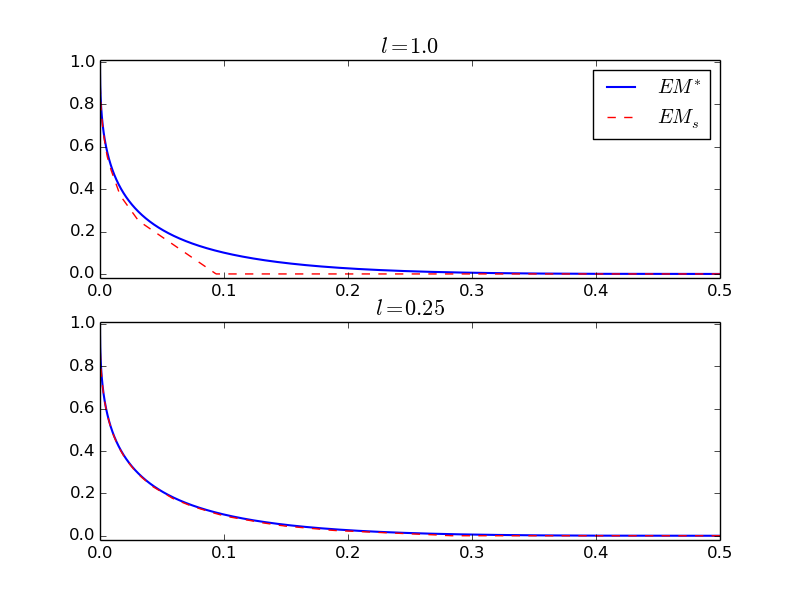
\includegraphics[width=\linewidth]{fig_source/EM-EMS.png}
\caption{Optimal and realized EM curves} %la légende
\label{aistat:EMMS}
\end{center}
\end{minipage}
\hfill
\begin{minipage}[c]{.5\linewidth}
\begin{center}
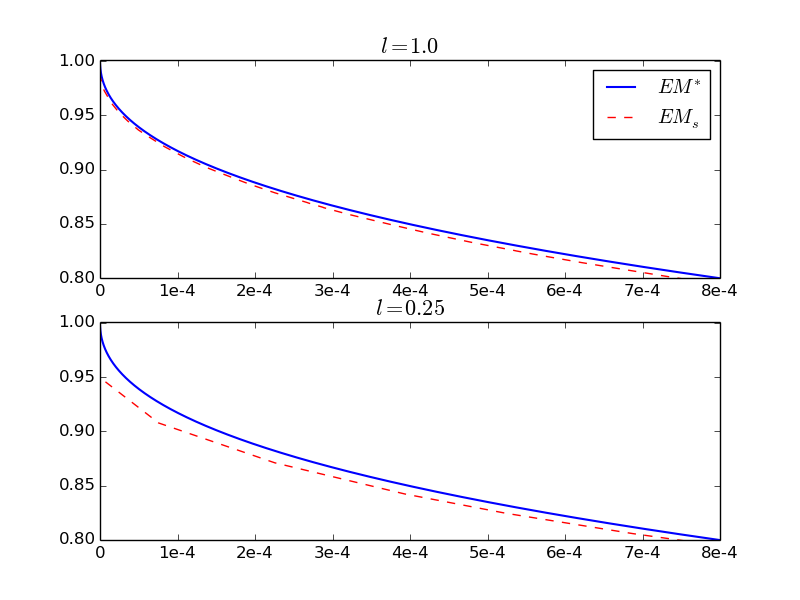
\includegraphics[width=\linewidth]{fig_source/EM-EMSzoom.png}
\caption{Zoom near 0 ~~~~~~~~~~~~~~~~~~~~~~~~~~~~~~~~~~~~~~~~~~~~~~~~~} %la légende
\label{aistat:EMMSzoom}
\end{center}
\end{minipage}
\end{figure}


\begin{figure}[!ht]
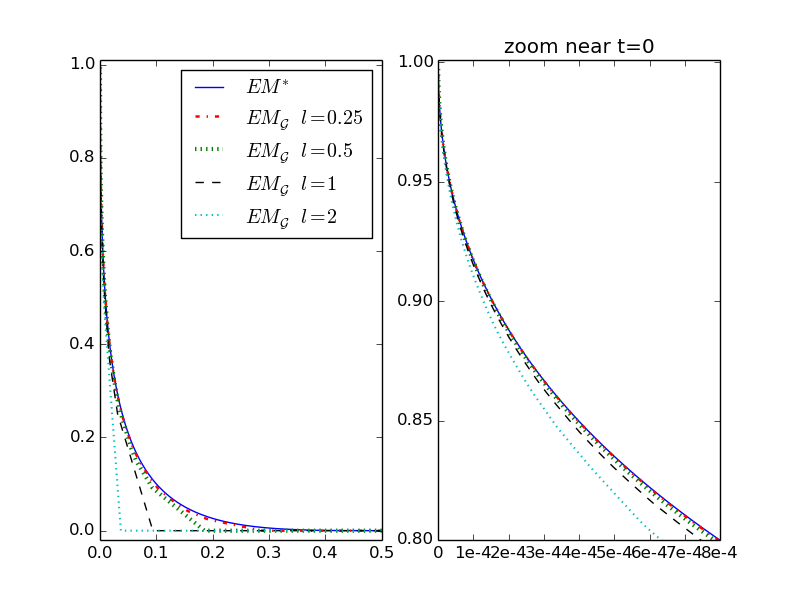
\includegraphics[width=\linewidth]{fig_source/EMG-EM.png}
\caption{$EM_\mathcal{G}$ for different $l$} %la légende
\label{aistat:EMGEM}
\end{figure}


\section{Conclusion}
Prolongating the contribution of \cite{CLEM13}, this chapter provides an alternative view (respectively, an other parameterization) of the anomaly scoring problem, leading to another adaptive method to build scoring functions, which offers theoretical and computational advantages both at the same time. This novel formulation yields a procedure producing a nested sequence of empirical density level sets, and exhibits a good performance, even in the non compact support case. 
Thus, the main drawbacks of the mass-volume curve criterion listed in the introduction section are resolved exepting drawback \textbf{1)}. In addition, the model bias has been incorporated in the rate bound analysis.
%
However, the use of the Excess-Mass criterion to measure the quality of a scoring function $s_n$ involves the computation of the Lebesgue measure  $\leb(s_n \ge u)$, just as with the Mass-Volume criterion (drawback \textbf{1)}). This is a major drawback for its use in high dimensional framework, if no prior knowledge on the form of these level sets is available.


\section{Illustrations}

Note that the scoring function we built in Algorithm~\ref{aistat:algo1} is incidentally an estimator of the density $f$ (usually called the silhouette), since $f(x)=\int_{0}^\infty \mathds{1}_{f \ge t}dt=\int_{0}^\infty \mathds{1}_{\Omega^*_t}dt$ and $s(x):= \sum_{k=1}^K (t_k-t_{k-1}) \mathds{1}_{x \in \hat{\Omega}_{t_k} }$ which is a discretization of $\int_{0}^\infty \mathds{1}_{\hat \Omega_t}dt$. This fact is illustrated in Figure~\ref{aistat:scoring3D}. Note that the silhouette does not focuse on local properties of the density, but only on its induced pre-order (level sets).
\begin{figure}[!h!]
\centering
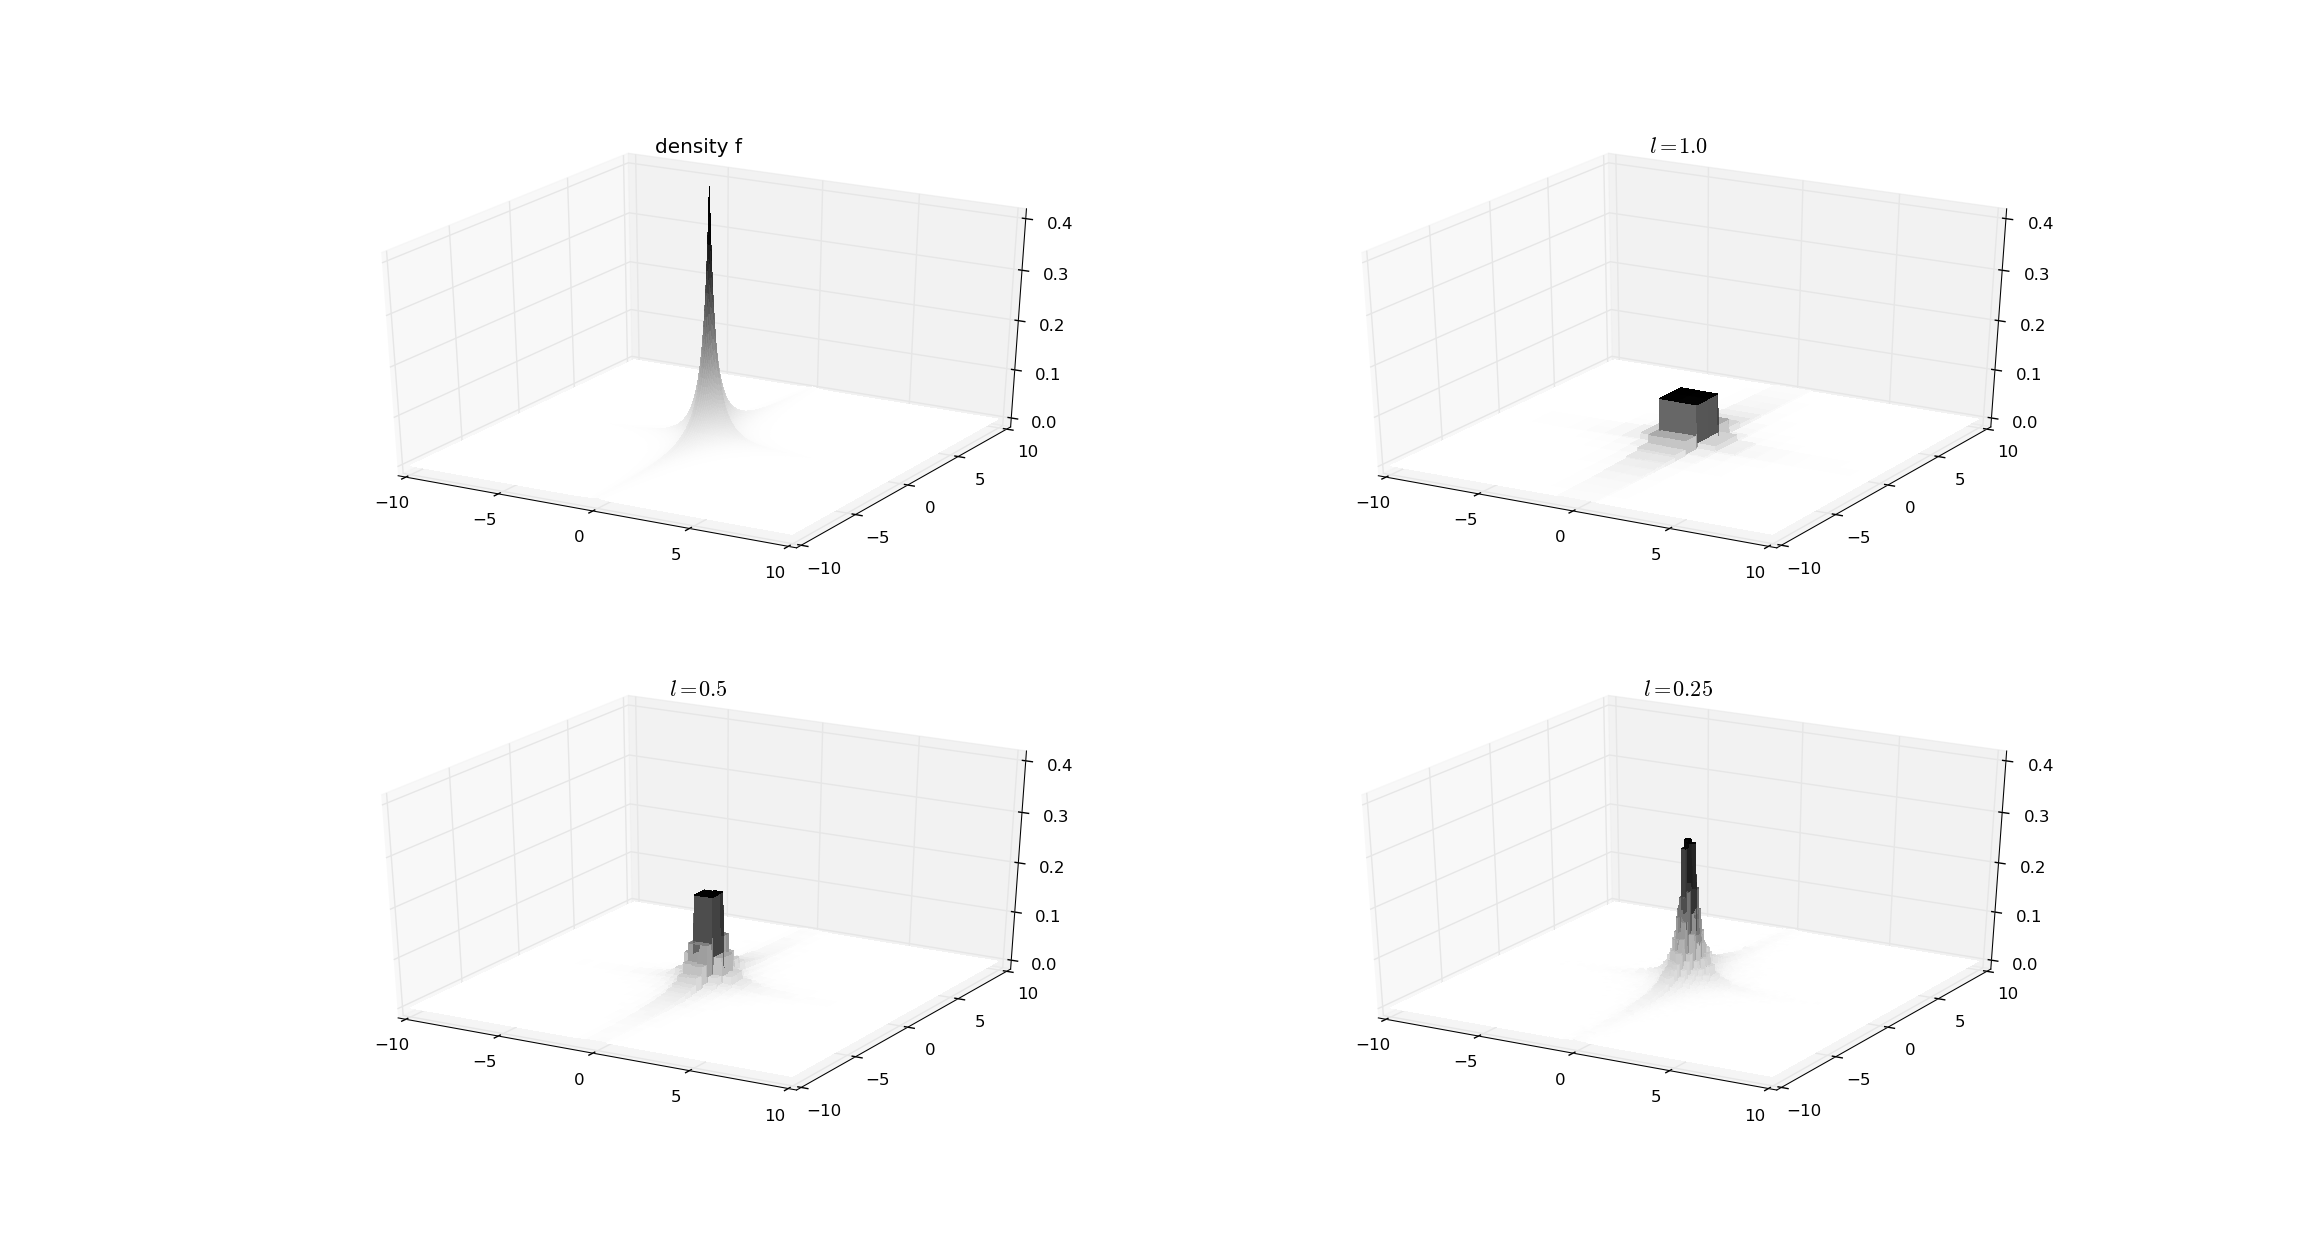
\includegraphics[width=\linewidth]{fig_source/scoring3D.png}
\caption{density and scoring functions} %la légende
\label{aistat:scoring3D}
\end{figure}






\section{Detailed Proofs}
\label{aistat:sec:detailed_proofs}
\subsection*{Proof of Proposition~\ref{aistat:derive}} Let $t>0$. Recall that $EM^{*}(t)=\alpha(t)-t \lambda(t)$ where $\alpha(t)$ denote the mass at level $t$, namely $\alpha(t)=\mathbb{P}(f(X) \ge t)$, and $\lambda(t)$ denote the volume at level $t$, i.e. $\lambda(t)=\leb(\{x, f(x) \ge t\})$. For $h>0$, let $A(h)$ denote the quantity $$A(h)=\frac{1}{h}(\alpha(t+h)-\alpha(t))$$ and $$B(h)=\frac{1}{h} (\lambda(t+h)-\lambda(t)).$$ It is straightforward to see that $A(h)$ and $B(h)$ converge when $h \rightarrow 0$, and expressing $EM^{*'}=\alpha'(t)-t\lambda'(t)-\lambda(t)$, it suffices to show that $\alpha'(t)-t\lambda'(t)=0$, namely $\lim_{h \rightarrow 0} A(h) - t~B(h) = 0$. Yet, we have $$A(h)-t~B(h)~=~\frac{1}{h} \int_{t \le f \le t+h}f-t ~\le~ \frac{1}{h} \int_{t \le f \le t+h} h  ~=~ \leb(t \le f \le t+h) \rightarrow 0$$ because $f$ has no flat part.


\subsection*{Proof of Lemma~\ref{aistat:evident}:}

On the one hand, for every $\Omega$ measurable, 
\begin{align*}
\mathbb{P}(X \in \Omega)-t~\leb(\Omega)&=\int_\Omega(f(x)-t)dx \\&\le \int_{\Omega \cap \{ f \ge t\}}(f(x)-t)dx \\&\le \int_{\{f \ge t\}}(f(x)-t)dx\\&=\mathbb{P}(f(X) \ge t)-t~\leb(\{ f \ge t\}).
\end{align*}
\noindent
It follows that $\{ f \ge t\} \in \arg\max_{A meas.}\mathbb{P}(X \in A)-t~\leb(A) $.\\

On the other hand, suppose $\Omega \in \arg\max_{A~ meas.}\mathbb{P}(X \in A)-t~\leb(A)$ and $\leb(\{f>t\} \setminus \Omega)>0$. Then there is $\epsilon > 0$ such that $\leb(\{f>t+\epsilon\} \setminus \Omega)>0$ (by sub-additivity of Leb, if it is not the case, then $ \leb(\{f>t\} \setminus \Omega) = \leb(\cup_{\epsilon \in \mathbb{Q}_+}\{ f>t+\epsilon\} \setminus \Omega)=0$ ). We have thus $$\int_{\{f>t\} \setminus \Omega} (f(x)-t)dx > \epsilon.\leb(\{f > t+ \epsilon\} \setminus \Omega) > 0~,$$ so that 
\begin{align*}
\int_{\Omega}(f(x)-t)dx &~\le~ \int_{ \{f>t\} }(f(x)-t)dx ~-~ \int_{ \{f>t \} \setminus \Omega}(f(x)-t)dx \\
&~<~ \int_{\{f>t\}}(f(x)-t)dx~,
\end{align*}

 i.e  
\begin{align*}
\mathbb{P}(X \in \Omega)-t~\leb(\Omega) ~~<~~ \mathbb{P}(f(X) \ge t) - t~\leb(\{x,f(x) \ge t\})   
\end{align*}
which is a contradiction. Thus, $\{f>t\} \subset \Omega$ Leb-almost surely.

To show that $ \Omega^*_t \subset \{x, f(x) \ge t\}$, suppose that $\leb(\Omega^*_t \cap \{f<t\}) > 0$. Then by sub-additivity of Leb just as above, there is $\epsilon >0$ such that $\leb(\Omega^*_t \cap \{f<t-\epsilon\}) > 0$ and $$\int_{\Omega^*_t \cap \{f<t-\epsilon\}} f-t \le -\epsilon.\leb(\Omega^*_t \cap \{f<t-\epsilon\})<0.$$ It follows that $$\mathbb{P}(X \in \Omega^*_t)-t~\leb(\Omega^*_t) < \mathbb{P}(X \in \Omega^*_t \setminus \{f<t-\epsilon\})-t~\leb(\Omega^*_t \setminus \{f<t-\epsilon\}),$$ which is a contradiction with the optimality of $\Omega_t^*$.



\subsection*{Proof of Proposition~\ref{aistat:propestim}}
Proving the first assertion is immediate, since $\int_{f \ge t}(f(x)-t)dx \ge \int_{s \ge t}(f(x)-t)dx$.
Let us now turn to the second assertion. We have:
\begin{align*}
EM^*(t)-EM_s(t)&=\int_{f>t}(f(x)-t)dx~-~\sup_{u>0}\int_{s>u}(f(x)-t)dx\\
&=\inf_{u>0} \int_{f>t}(f(x)-t)dx     ~-~\int_{s>u}(f(x)-t)dx~.
\end{align*}
Yet,
\begin{align*}
&\int_{\{f>t\}\setminus\{s>u\}}(f(x)-t)dx + \int_{\{s>u\}\setminus\{f>t\}}(t-f(x))dx\\
&~~~~~~~~~~~~~~~~~~~~~~~~~~~~~~~~\le (\|f\|_\infty-t).\leb\Big(\{f>t\} \setminus \{s>u\}\Big)~+~ t~\leb\Big(\{s>u\} \setminus \{f>t\}\Big),
\end{align*}
 so we obtain:
\begin{align*}
EM^*(t)-EM_s(t)  &\le~ \max(t,\|f\|_\infty-t) ~~\leb\Big(\{s>u\} \Delta \{f>t\}\Big) \\
&\le~ \|f\|_\infty .\leb\Big(\{s>u\} \Delta \{f>t\}\Big) .
\end{align*}

\noindent To prove the third point, note that:

\begin{align*}
\inf_{u>0} \leb\Big(\{s>u\} \Delta \{f>t\}\Big)~=~\inf_{T \nearrow} \leb\Big(\{Ts>t\} \Delta \{f>t\}\Big)  
\end{align*}

Yet,
\begin{align*} 
\leb\Big(\{Ts> t\} \Delta \{f>t\}\Big) &\le{\leb(\{f>t-\|Ts-f\|_\infty\} \smallsetminus \{f>t+\|Ts-f\|_\infty\})}\\
&=\lambda(t-\|Ts-f\|_\infty)~-~\lambda(t+\|Ts-f\|_\infty)\\
&=-\int_{t-\|Ts-f\|_\infty}^{t+\|Ts-f\|_\infty}\lambda'(u)du ~.
\end{align*}
\noindent
On the other hand, we have $\lambda(t)=\int_{\mathbb{R}^d}\mathds{1}_{f(x)\ge t}dx = \int_{\mathbb{R}^d} g(x) \|\nabla f(x)\|dx$, where we let $$g(x) = \frac{1}{\|\nabla f(x)\|} \mathds{1}_{\{x,\|\nabla f(x)\|>0, f(x)\ge t\}}.$$ The co-area formula (see \cite{Federer1969}, p.249, th.3.2.12) gives in this case: $$\lambda(t)=\int_{\mathbb{R}} du \int_{f^{-1}(u)}\frac{1}{\|\nabla f(x)\|} \mathds{1}_{\{x,f(x)\ge t\}}d\mu (x) = \int_{t}^\infty du \int_{f^{-1}(u)}\frac{1}{\|\nabla f(x)\|}d\mu (x)$$ so that $\lambda'(t)=-\int_{f^{-1}(u)}\frac{1}{\|\nabla f(x)\|}d\mu (x)$.\\

\noindent Let $\eta_\epsilon$ such that $ \forall u > \epsilon,~|\lambda'(u)|= \int_{f^{-1}(u)} \frac{1}{\|\nabla f(x)\|} d\mu(x)<\eta_\epsilon$.
 We obtain:
\begin{align*}
\sup_{t \in [\epsilon + \inf_{T \nearrow}\|f-Ts\|_\infty,\|f\|_\infty]} EM^*(t)-EM_s(t)~\le~ 2.\eta_\epsilon.\|f\|_\infty \inf_{T \nearrow}\|f-Ts\|_\infty.
\end{align*}
\noindent In particular, if $\inf_{T \nearrow}\|f-Ts\|_\infty \le \epsilon_1 $, 
 $$\sup_{[\epsilon + \epsilon_1,\|f\|_\infty]}|EM^*-EM_s| \le 2.\eta_{\epsilon}.\|f\|_\infty. \inf_{T \nearrow}\|f-Ts\|_\infty~. $$
\noindent


\subsection*{Proof of Proposition~\ref{aistat:propmono}}


\noindent Let $i$ in $\{1,...,K\}$. First, note  that:
\begin{align*}
H_{n,t_{i+1}}(\hat \Omega_{t_{i+1}} \cup \hat \Omega_{t_{i}}) &~=~ H_{n,t_{i+1}}(\hat \Omega_{t_{i+1}}) ~+~ H_{n,t_{i+1}}(\hat \Omega_{t_{i}} \smallsetminus \hat \Omega_{t_{i+1}}),\\
H_{n,t_{i}}(\hat \Omega_{t_{i+1}} \cap \hat \Omega_{t_{i}}) &~=~ H_{n,t_{i}}(\hat \Omega_{t_{i}}) - H_{n,t_{i}}(\hat \Omega_{t_{i}} \smallsetminus \hat \Omega_{t_{i+1}}).
\end{align*}
It follows that
\begin{align*}
&H_{n,t_{i+1}}( \hat \Omega_{t_{i+1}} \cup \hat \Omega_{t_{i}}) ~+~ H_{n,t_{i}}(\hat \Omega_{t_{i+1}} \cap \hat \Omega_{t_{i}}) \\
&~~~~~~~~~~~~~~~~~~~=~~ H_{n,t_{i+1}}(\hat \Omega_{t_{i+1}}) ~+~ H_{n,t_{i}}(\hat \Omega_{t_{i}}) ~+~ H_{n,t_{i+1}}(\hat \Omega_{t_{i}} \setminus \hat \Omega_{t_{i+1}}) ~-~ H_{n,t_{i}}(\hat \Omega_{t_{i}} \setminus \hat \Omega_{t_{i+1}})~,
\end{align*}
with $H_{n,t_{i+1}}(\hat \Omega_{t_{i}} \setminus \hat \Omega_{t_{i+1}}) - H_{n,t_{i}}(\hat \Omega_{t_{i}} \setminus \hat \Omega_{t_{i+1}}) \ge 0$ since $H_{n,t}$ is decreasing in $t$. But on the other hand, by definition of $\hat \Omega_{t_{i+1}}$ and $\hat \Omega_{t_{i}}$ we have:
\begin{align*}
H_{n,t_{i+1}}(\hat \Omega_{t_{i+1}} \cup \hat \Omega_{t_{i}}) &~~\le~~ H_{n,t_{i+1}}(\hat \Omega_{t_{i+1}})\,,\\
H_{n,t_{i}}(\hat \Omega_{t_{i+1}} \cap \hat \Omega_{t_{i}}) &~~\le~~ H_{n,t_{i}}(\hat \Omega_{t_{i}})\,.
\end{align*}
\noindent
Finally we get:
\begin{align*}
H_{n,t_{i+1}}(\hat \Omega_{t_{i+1}} \cup \hat \Omega_{t_{i}}) &~~=~~ H_{n,t_{i+1}}(\hat \Omega_{t_{i+1}})\,,\\
H_{n,t_{i}}(\hat \Omega_{t_{i+1}} \cap \hat \Omega_{t_{i}}) &~~=~~ H_{n,t_{i}}(\hat \Omega_{t_{i}})\,.
\end{align*}

\noindent
Proceeding by induction we have, for every $m$ such that $k+m \le K$:
\begin{align*}
H_{n,t_{i+m}}(\hat \Omega_{t_i} \cup \hat \Omega_{t_{i+1}} \cup ... \cup \hat \Omega_{t_{i+m}}) &~~=~~ H_{n,t_{i+m}}(\hat \Omega_{t_{i+m}})~,\\
H_{n,t_i}(\hat \Omega_{t_i} \cap \hat \Omega_{t_{i+1}} \cap ... \cap \hat \Omega_{t_{i+m}}) &~~=~~ H_{n,t_i}(\hat \Omega_{t_i})~.
\end{align*}
Taking (i=1, m=k-1) for the first equation and  (i=k, m=K-k) for the second completes the proof.\\



\subsection*{Proof of Theorem~\ref{aistat:compact_support_case}}

We shall use the following lemma:
\begin{lemma}
\label{aistat:lemmeMs}
With probability at least $1-\delta$, for $k \in \{1,...,K\}$, $$0 ~~\le~~ EM^*(t_{k})-EM_{s_K}(t_k) ~~\le~~ 2 \Phi_n(\delta).$$ 
\end{lemma}
\noindent

\textbf{Proof of Lemma~\ref{aistat:lemmeMs}: } 

Remember that by definition of $\hat \Omega_{t_k}$: $H_{n,t_k}(\hat \Omega_{t_k})=\max_{\Omega \in \mathcal{G}} H_{n,t_k}(\Omega) $ and note that:
$$EM^*(t_k)=\max_{\Omega~ meas.} H_{t_k}(\Omega)=\max_{\Omega \in \mathcal{G}} H_{t_k}(\Omega) ~~\ge~~ H_{t_k}(\hat \Omega_{t_k}). $$

%\begin{align}
%&\label{aistat:aa} \gamma(t_k)=\max_{\Omega~ meas.} \mathbb{P}(X \in \Omega) - t_k.\leb(\Omega)=\max_{\Omega~ \in \mathcal{G}} \mathbb{P}(X \in \Omega) - t_k.\leb(\Omega) \mbox{~~(by \textbf{A5})~~} \\
%&\label{aistat:bb} \gamma(t_k) ~\geq~ \beta(t_k):= \mathbb{P}(X\in \hat \Omega_{t_k})-t_k.\leb(\hat \Omega_{t_k})\\
%&\label{aistat:cc} \hat \gamma (t_k)~=~ \mathbb{P}_n(X \in \hat \Omega_{t_k})-t_k.\leb(\hat \Omega_{t_k}) ~=~ \max_{\Omega \in \mathcal{G}} ~~\mathbb{P}_n(X \in \Omega)-t_k.\leb(\Omega)
%\end{align}
On the other hand, using (\ref{aistat:penality}),  with probability at least $1-\delta$, for every $G \in \mathcal{G},~ |\mathbb{P}(G)-\mathbb{P}_n (G)| \leq \Phi_n(\delta)$. 
Hence, with probability at least $1-\delta$, for all $\Omega \in \mathcal{G}$ :
\begin{align*}
H_{n,t_k}(\Omega)-\Phi_n(\delta) ~~\le~~ H_{t_k}(\Omega) ~~\le~~ H_{n,t_k}(\Omega) + \Phi_n(\delta)
\end{align*}
\noindent so that, with probability at least $(1-\delta)$, for $k \in \{1..,K\}$,
\begin{align*}
H_{n,t_k}(\hat \Omega_{t_k})-\Phi_n(\delta) ~~\le~~ H_{t_k}(\hat \Omega_{t_k}) 
 ~~\le~~ EM^*(t_k) 
~~\le~~ H_{n,t_k}(\hat \Omega_{t_k}) + \Phi_n(\delta) ~,
\end{align*}
\noindent whereby, with probability at least $(1-\delta)$, for $k \in \{1,..,K\}$,
\begin{align*}
0 ~~\le~~ EM^*(t_k) - H_{t_k}(\hat \Omega_{t_k}) ~~\le~~ 2 \Phi_n(\delta)~.
\end{align*}


The following Lemma is a consequence of the derivative property of $EM^*$ (Proposition~\ref{aistat:derive}) 
% : the fact that $EM^{*'}=- \lambda$ (proposition~\ref{aistat:derive}) and that $\lambda$ is a decreasing function.
\begin{lemma}
\label{aistat:lemmederive}
Let $k$ in $\{1,...,K-1\}$. Then for every $t$ in $]t_{k+1},t_{k}]$,
$$0 ~~\le~~ EM^*(t)-EM^*(t_{k}) ~~\le~~ \lambda(t_{k+1}) (t_{k}-t_{k+1}).$$
\end{lemma}

\noindent Combined with Lemma~\ref{aistat:lemmeMs} and the fact that $EM_{s_K}$ is non-increasing, and writing 
\begin{align*}
EM^*(t)-EM_{s_K}(t) ~~=~~ (EM^*(t)-EM^*(t_k)) &~+~ (EM^*(t_k) ~-~ EM_{s_K}(t_k)) \\&~+~ (EM_{s_K}(t_k) ~-~ EM_{s_K}(t))
\end{align*}
this result leads to:
\begin{align*}
\forall k \in~ \{0,...,K-1\},&~ \forall t \in~ ]t_{k+1},t_{k}],
\\& ~~~~~~~~~~~~~~0 ~~\le~~ EM^*(t)-EM_{s_K}(t) ~~\le~~ 2 \Phi_n(\delta)+\lambda(t_{k+1})(t_{k}-t_{k+1}) 
\end{align*}
which gives Lemma~\ref{aistat:theofini} stated in the sketch of proof. Notice that we have not yet used the fact that $f$ has a compact support.
%and in particular, for $t \in~ ]t_{K},t_{1}]$, $|EM^*(t)-EM_{s_K}(t)| \le 2 \Phi_n(\delta)+\lambda(t_{K})\max_{k=1..K}(t_{k}-t_{k+1})$. The theorem follows directly from these arguments.

%Note in particular that with probability at least $1-\delta$, we have for all $t$ in $]t_{K},t_{1}]$:
%\begin{equation*}
%|EM^*(t)-EM_{s_K}(t)| \leq  \left(A+\sqrt{2log(1/\delta)}\right)\frac{1}{\sqrt n} + \lambda(t_{K})\sup_{1\leq k< K}(t_{k}-t_{k+1}).
%\end{equation*}

The compactness support assumption allows an extension of Lemma~\ref{aistat:lemmederive} to $k=K$, namely the inequality holds true for $t$ in $]t_{K+1},t_K]=]0,t_K]$ as soon as we let $\lambda(t_{K+1}):=\leb(supp f)$. Indeed the compactness of $supp f$ implies that $\lambda(t) \rightarrow \leb(supp f)$ as $t \rightarrow 0$. Observing that Lemma~\ref{aistat:lemmeMs} already contains the case $k=K$, this leads to, for $k$ in $\{0,...,K\}$ and $t \in~ ]t_{k+1},t_{k}],~ |EM^*(t)-EM_{s_K}(t)| \le 2 \Phi_n(\delta)+\lambda(t_{k+1})(t_{k}-t_{k+1})$. Therefore, $\lambda$ being a decreasing function bounded by $\lambda(\leb(supp f))$, we obtain the following: with probability at least $1-\delta$, we have for all $t$ in $]0,t_{1}]$,
\begin{align*}
|EM^*(t)-EM_{s_K}(t)| 
~~\le~~  \left(A+\sqrt{2log(1/\delta)}\right)\frac{1}{\sqrt n}~+~ \lambda(\leb(supp f))\sup_{1\leq k \le K}(t_{k}-t_{k+1}).
\end{align*}

%Observe that $\lambda$ is a decreasing function majored by $\leb(\supp f)$. 
%For $\epsilon > 0$, let $E_\epsilon$ denote the event \{$\sup_{t \in ]t_{K},t_{1}]} |EM^*(t)-EM_{s_K}(t)| \le (A+\sqrt{2\log(1/\delta)}+\leb(\supp f))\frac{1}{\sqrt{n}}$\}.
%We have $\mathbb{P}(E_\epsilon) \ge 1-\delta$ and the $(E_\epsilon)_\epsilon$ are decreasing sets (for inclusion) when $\epsilon$ is decreasing, so that we can make $\epsilon \rightarrow 0$ to obtain Theorem~\ref{aistat:compact_support_case}.


\subsection*{Proof of Theorem~\ref{aistat:thmprinc}}
\noindent
The first part of this theorem is a consequence of (\ref{aistat:fondineq}) combined with:
\begin{align*}
\sup_{t \in ]0,t_N]} |EM^*(t)-EM_{s_N}(t)| ~\le~ 1-EM_{s_N}(t_N) ~~\le~~ 1-EM^*(t_N)+2\Phi_n(\delta)~,
\end{align*} 
where we use the fact that $0 \le EM^*(t_N)-EM_{s_N}(t_N) \le 2 \Phi_n(\delta)$ following from Lemma~\ref{aistat:lemmeMs}.\\
\noindent To see the convergence of $s_N(x)$, note that:

\begin{align*}
s_N(x)~=~\frac{t_1}{\sqrt n} \sum_{k=1}^{\infty}\frac{1}{(1+\frac{1}{\sqrt n})^k} \mathds{1}_{x \in \hat \Omega_{t_k}} \mathds{1}_{\{k \le N\}}~~\le~~ \frac{t_1}{\sqrt n} \sum_{k=1}^{\infty} \frac{1}{(1+\frac{1}{\sqrt n})^k} ~<~ \infty,
\end{align*}

and analogically to Remark~\ref{aistat:orderscore} observe that $EM_{s_N} \le EM_{s_\infty}$ so that $\sup_{t \in ]0,t_1]} |EM^*(t)-EM_{s_\infty}(t)| \leq \sup_{t \in ]0,t_1]} |EM^*(t)-EM_{s_N}(t)|$ which prooves the last part of the theorem.

\subsection*{Proof of Lemma~\ref{aistat:propbiais}}

By definition, for every class of set $\mathcal{H}$, $EM_{\mathcal{H}}^*(t)=\max_{\Omega \in \mathcal{H}}H_t(\Omega)$.
The bias $ EM^*(t)-EM^*_{\mathcal{G}}(t)$ of the model $\mathcal{G}$ is majored by $ EM^*(t)-EM^*_{\mathcal{F}}(t)$ since $\mathcal{F} \subset \mathcal{G}$.
\noindent Remember that $$f_{F}(x) := \sum_{i \ge 1} \mathds{1}_{x \in F_i} \frac{1}{|F_i|} \int_{F_i}f(y)dy,$$ and note that for all $t>0$, $\{ f_{F} > t \} \in \mathcal{F}$. It follows that:
\begin{align*}
EM^*(t)-EM^*_{\mathcal{F}}(t) &~~=~~ \int_{f>t}(f-t)- \sup_{C \in \mathcal{F} }\int_{C}(f-t) \\
\le&~~ \int_{f>t}(f-t)- \int_{f_{F} > t}(f-t) ~~~~~~~~~~~~~~~~~\mbox{~since~} \{f_{F} > t\} ~\in~ \mathcal{F}  \\
=&~~\int_{f>t}(f-t)- \int_{f_{F} > t}(f_{F}-t) ~~~~~~~~~~~~~~~\mbox{~since~} \forall G \in \mathcal{F}, \int_Gf=\int_Gf_{F}\\
=&~~\int_{f>t}(f-t)-\int_{f>t}(f_{F}-t)+\int_{f>t}(f_{F}-t)-\int_{f_{F} > t}(f_{F}-t)\\
=&~~\int_{f>t}(f-f_{F})+\int_{\{f>t\}\setminus \{f_{F}>t\}}(f_{F}-t)-\int_{\{f_{F}>t\} \setminus \{f>t\}}(f_{F}-t)~.
\end{align*}
\noindent Observe that the second and the third term in the bound are non-positive. Therefore:
\begin{align*}
EM^*(t)-EM^*_{\mathcal{F}}(t) \le \int_{f>t}(f-f_{F}) \le \int_{\mathbb{R}^d}|f-f_{F}|~.
\end{align*}
